\documentclass[8pt]{beamer}



\mode<presentation>
{
%  \usetheme{Berkeley}
	\usetheme{Dresden}
%	\usetheme{Berlin}
%   \usecolortheme{dove}
%   \usecolortheme{dolphin}
%   \useinnertheme{circles}
   
  \setbeamercovered{transparent}

}


\usepackage[english]{babel}
\usepackage[utf8]{inputenc}
\usepackage{times}
\usepackage[T1]{fontenc}
\usepackage{multimedia}
\usepackage[absolute,overlay]{textpos}
\usepackage{graphicx}

\usepackage{xcolor}
\usepackage{amsmath}
\usepackage[absolute,overlay]{textpos}
\usepackage{physics}
\usepackage{fixltx2e}
\usepackage{appendixnumberbeamer}
\usepackage{booktabs}

\graphicspath{{./media/images/}}

\definecolor{paint}{RGB}{150,0,0}
\setbeamercolor {structure} {fg=paint}
%\setbeamercolor{title}{fg=black}
%\setbeamertemplate{itemize items}[circle]




\newcommand{\jsqrt}[2]{\bqty{ #1 #1 | #2 #2 }}
\newcommand{\ksqrt}[2]{\bqty{ #1 #2 | #2 #1 }}
\newcommand\mf[1]{\mathbf{#1}}
\newcommand\dens{\rho(\mathbf{r})}
\newcommand\densin{\rho^{in}(\mathbf{r})}
\newcommand\densout{\rho^{out}(\mathbf{r})}
\newcommand\rdens{\tilde{\rho}(\mathbf{G})}
\newcommand\erre{\mathbf{r}}
\newcommand\GI{\mathbf{G}}
\newcommand\QE{\textsc{Quantum} ESPRESSO }
\newcommand\numbands{n_{bands}}
\newcommand\numG{n_{G}}
\newcommand\numR{n_{R}}
\newcommand\bigO{\mathcal{O}}
\newcommand\CO{Co\textsubscript{3}O\textsubscript{4} } 


\title[Tuning the computational architecture for Quantum Espresso \textit{ab initio} calculation of nanostructures] % (optional, use only with long paper titles)
{Tuning the computational architecture for Quantum Espresso \textit{ab initio} calculation of nanostructures}

\author[Giorgio Ruffa] 
{Giorgio Ruffa}
\institute[Università degli Studi di Milano]{Università degli Studi di Milano}

\date{28 Aprile 2016} 

\subject{}


\begin{document}

% ********** 1 slide *****************
\begin{frame}
  \titlepage
\end{frame}

\section{Introduzione}
\subsection{Density Functional Theory}
% ********** slide 2 *****************

\begin{frame}{}
\begin{columns}
	\column{0.33\textwidth}
		\begin{center}
			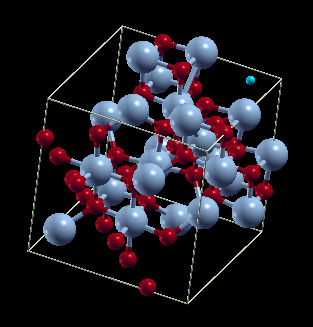
\includegraphics[height=3.5cm]{beam_co3.png}
		\end{center}
	\column{0.33\textwidth}
		\begin{center}
			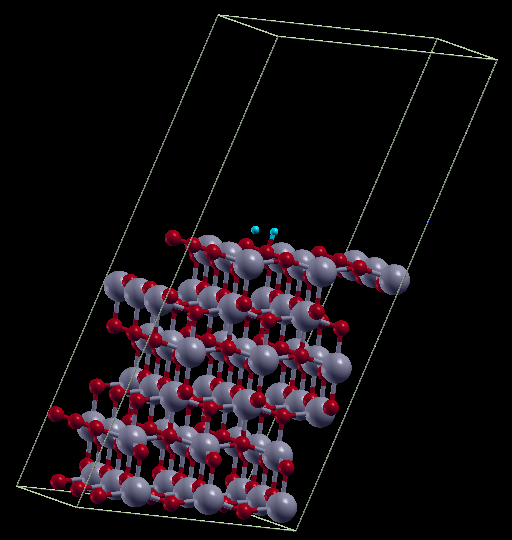
\includegraphics[height=3.5cm]{titania_crystal.png}
		\end{center}
	\column{0.33\textwidth}
		\begin{center}
			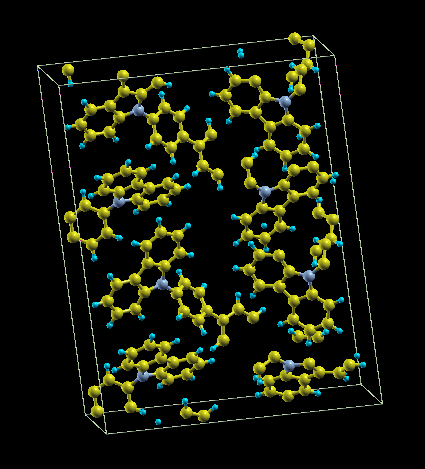
\includegraphics[height=3.5cm]{beam_cbp.png}
		\end{center}
\end{columns}
\begin{columns}
	\column{0.5\textwidth}
		\begin{center}
			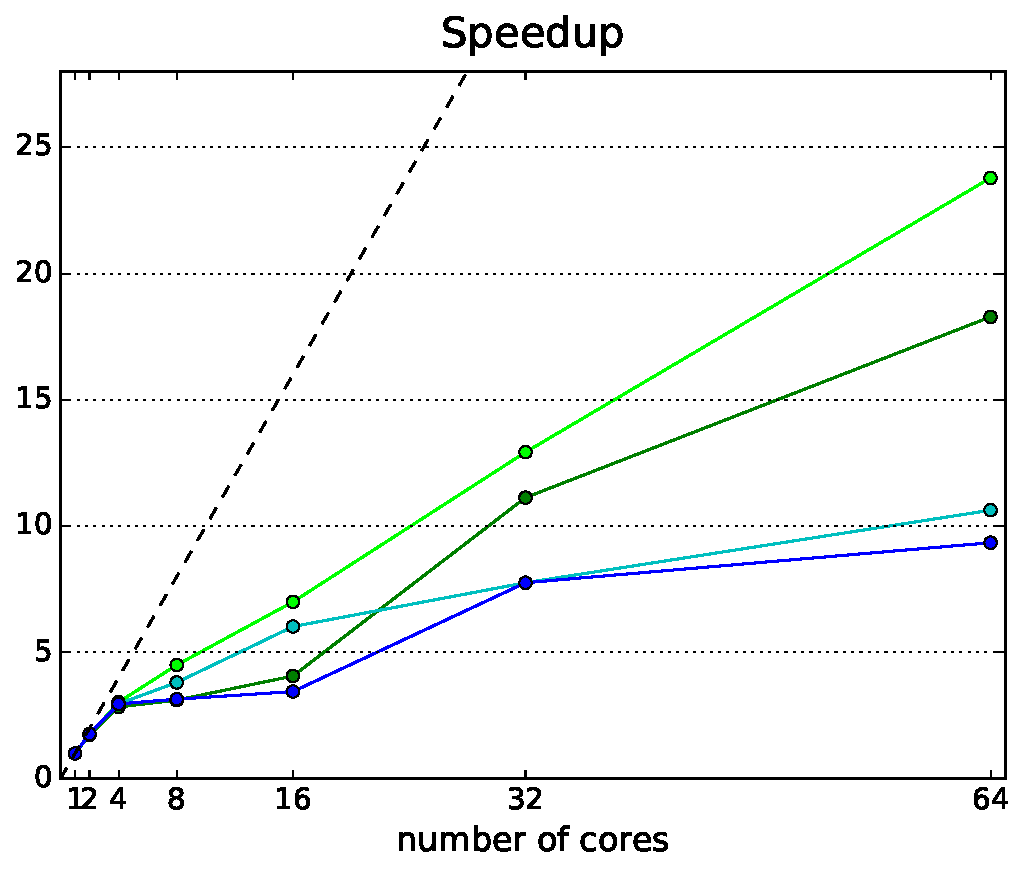
\includegraphics[height=3.5cm]{beam_first_slide.pdf}
		\end{center}
	\column{0.5\textwidth}
	\begin{block}{Outline}
		\begin{itemize}
			\item Teoria DFT
			\pause
			\item Implementazione PW SCF
			\pause
			\item Strategie di ottimizzazione
			\pause
			\item Miglioramento prestazioni
			\pause
			\item Conclusioni e scenari di utilizzo
		\end{itemize}
	\end{block}
\end{columns}
		
\end{frame}

% ********** slide 3 *****************
\begin{frame}{Introduzione}


\begin{columns}
	\column{0.5\textwidth}
%		\begin{center}
%			
\includegraphics[width=4cm]{beam_qe_logo.jpg}		
%		\end{center}
	
	\invisible<1>{\begin{block}{Density Functional Theory (DFT)}
		\begin{itemize}
			\setlength\itemsep{1em}
			\item[]<2-> Equazioni di Kohn-Sham :
			\item[]<2-> $ \displaystyle  \lbrace  - \frac{1}{2} \nabla^2+ v_{eff}(\erre) \rbrace 	\psi_{j}^{KS}(\erre) = \varepsilon_{j}^{KS} 	\psi_{j}^{KS}(\erre)$
			\item[]<3-> $ \displaystyle  v_{eff}(\erre) = v_{ion}(\erre) + v_{h}(\erre) + v_{xc}(\erre)$
			\item[]<3-> $ \displaystyle v_{h}(\erre) = \int \frac{\rho(\erre')}{\mid \erre - \erre'\mid} \dd{\erre'} $
			\item[]<3-> $ \displaystyle v_{xc}(\erre) =	\frac{\var{E_{xc}[\dens]}}{\var{\dens}}$
		\end{itemize}
	\end{block}}
		
	\column{0.5\textwidth}
		\begin{center}

			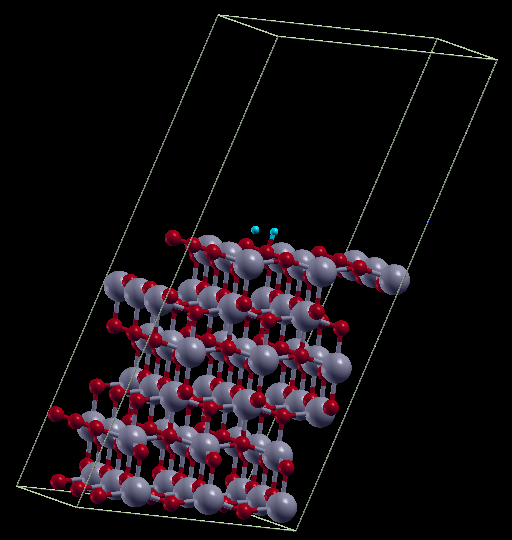
\includegraphics[width=3.5cm]{titania_crystal.png}	\\

			~ \\
			Superficie TiO\textsubscript{2} : \\ $ 150$ Atomi $\sim 2 \cdot 10 ^{3} e^{-}$	

		\end{center}
\end{columns}

\end{frame}

% ********** slide 4 *****************
\begin{frame}{Self Consistent DFT}
\begin{center}
	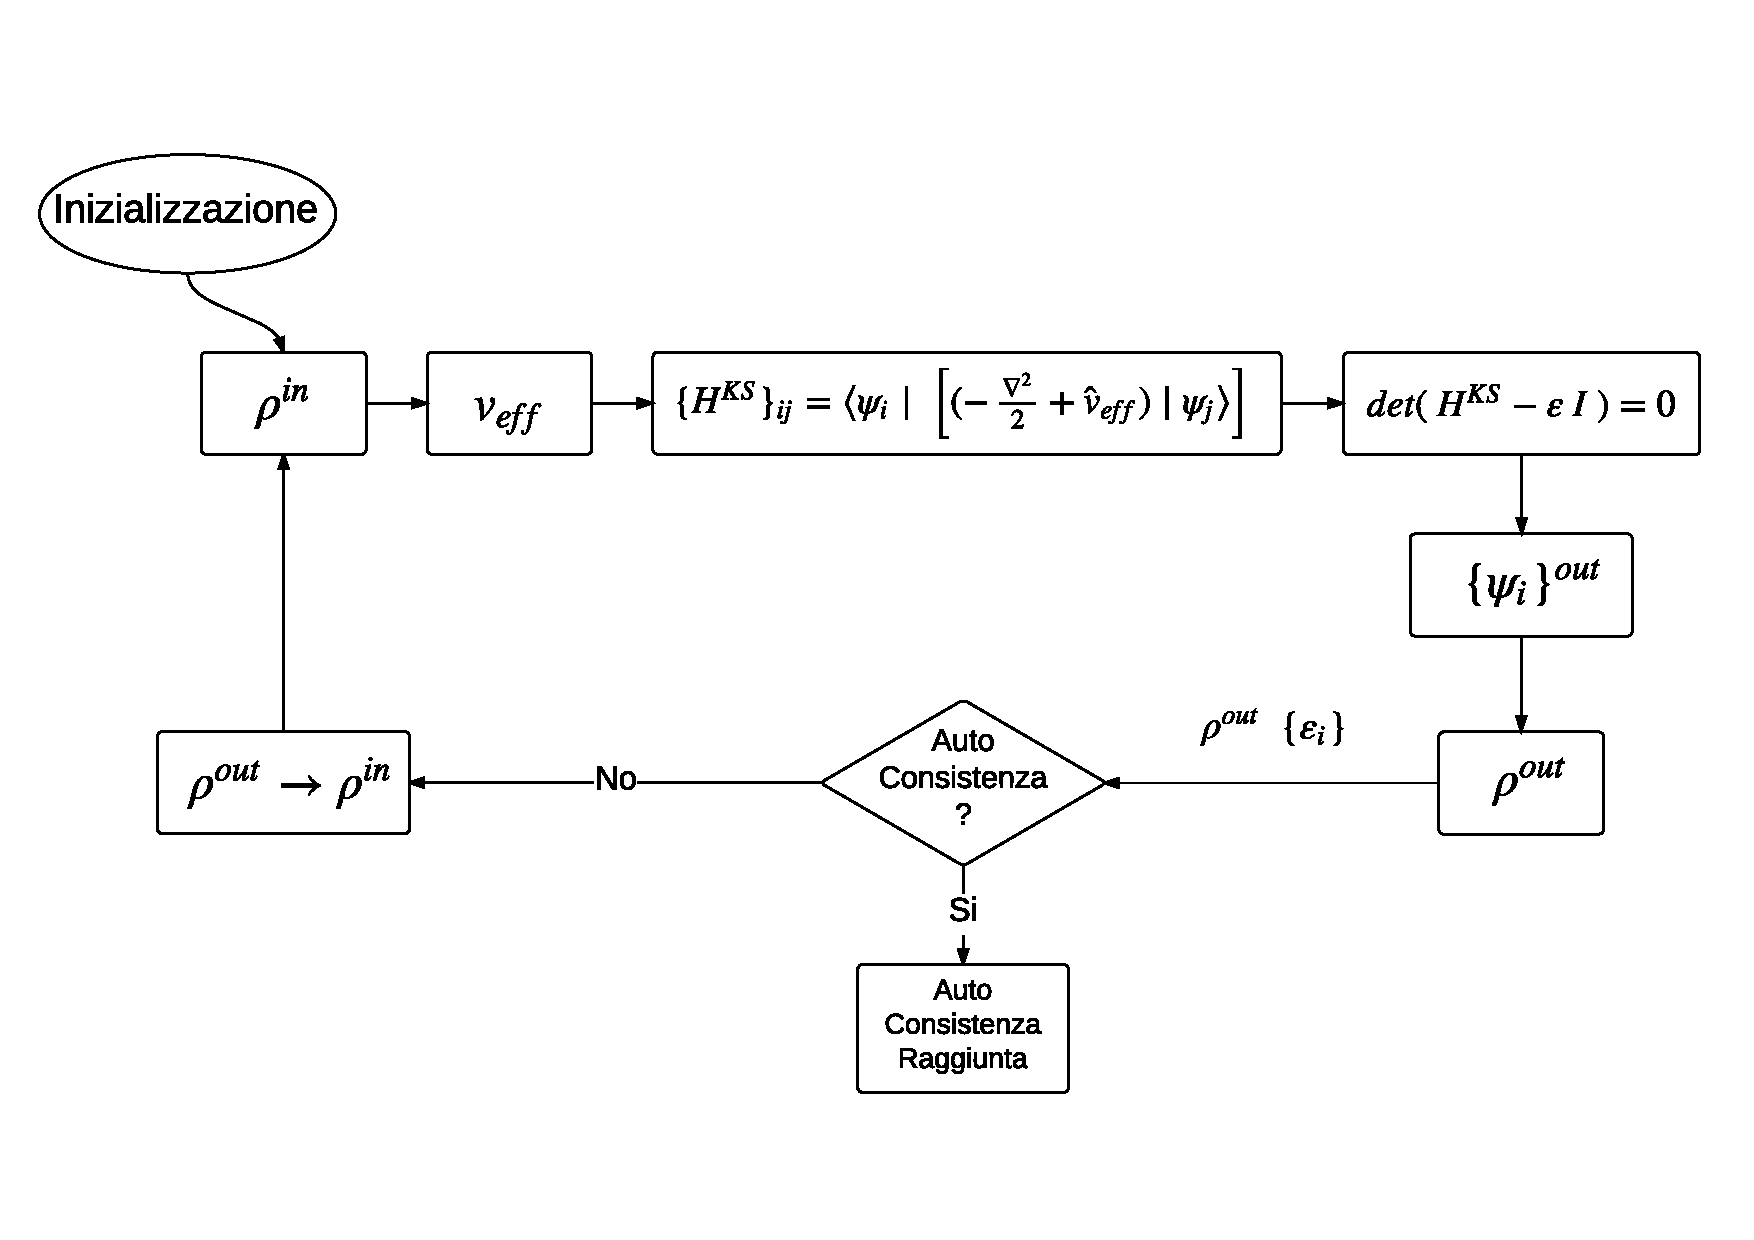
\includegraphics[width=\textwidth]{beam_SCF_0.pdf}	
\end{center}
\end{frame}

\section{Implementazione e Architetture}
\subsection{Implementazione e Architetture}

% ********** slide 5 *****************}

\def \inputPos {3}
\def \electronsPos {4}
\def \cegtergPos {5}
\def \hpsiPos {6}
\def \cdiaghgPos {7}
\def \sumbandPos {8}
\def \fftPos {9}
\def \fftscatterPos {10}
\def \scfPicWidth {1.1}
\def \scfPicHeight {0.62}

\begin{frame}{Funzioni rilevanti}
\vbox{
    \begin{minipage}[t][0.5\textheight][t]{\textwidth}
    	\begin{columns}
    		\column{0.5\textwidth}

			   \begin{flushleft}
			   	\only<1,\fftPos,\fftscatterPos>{
					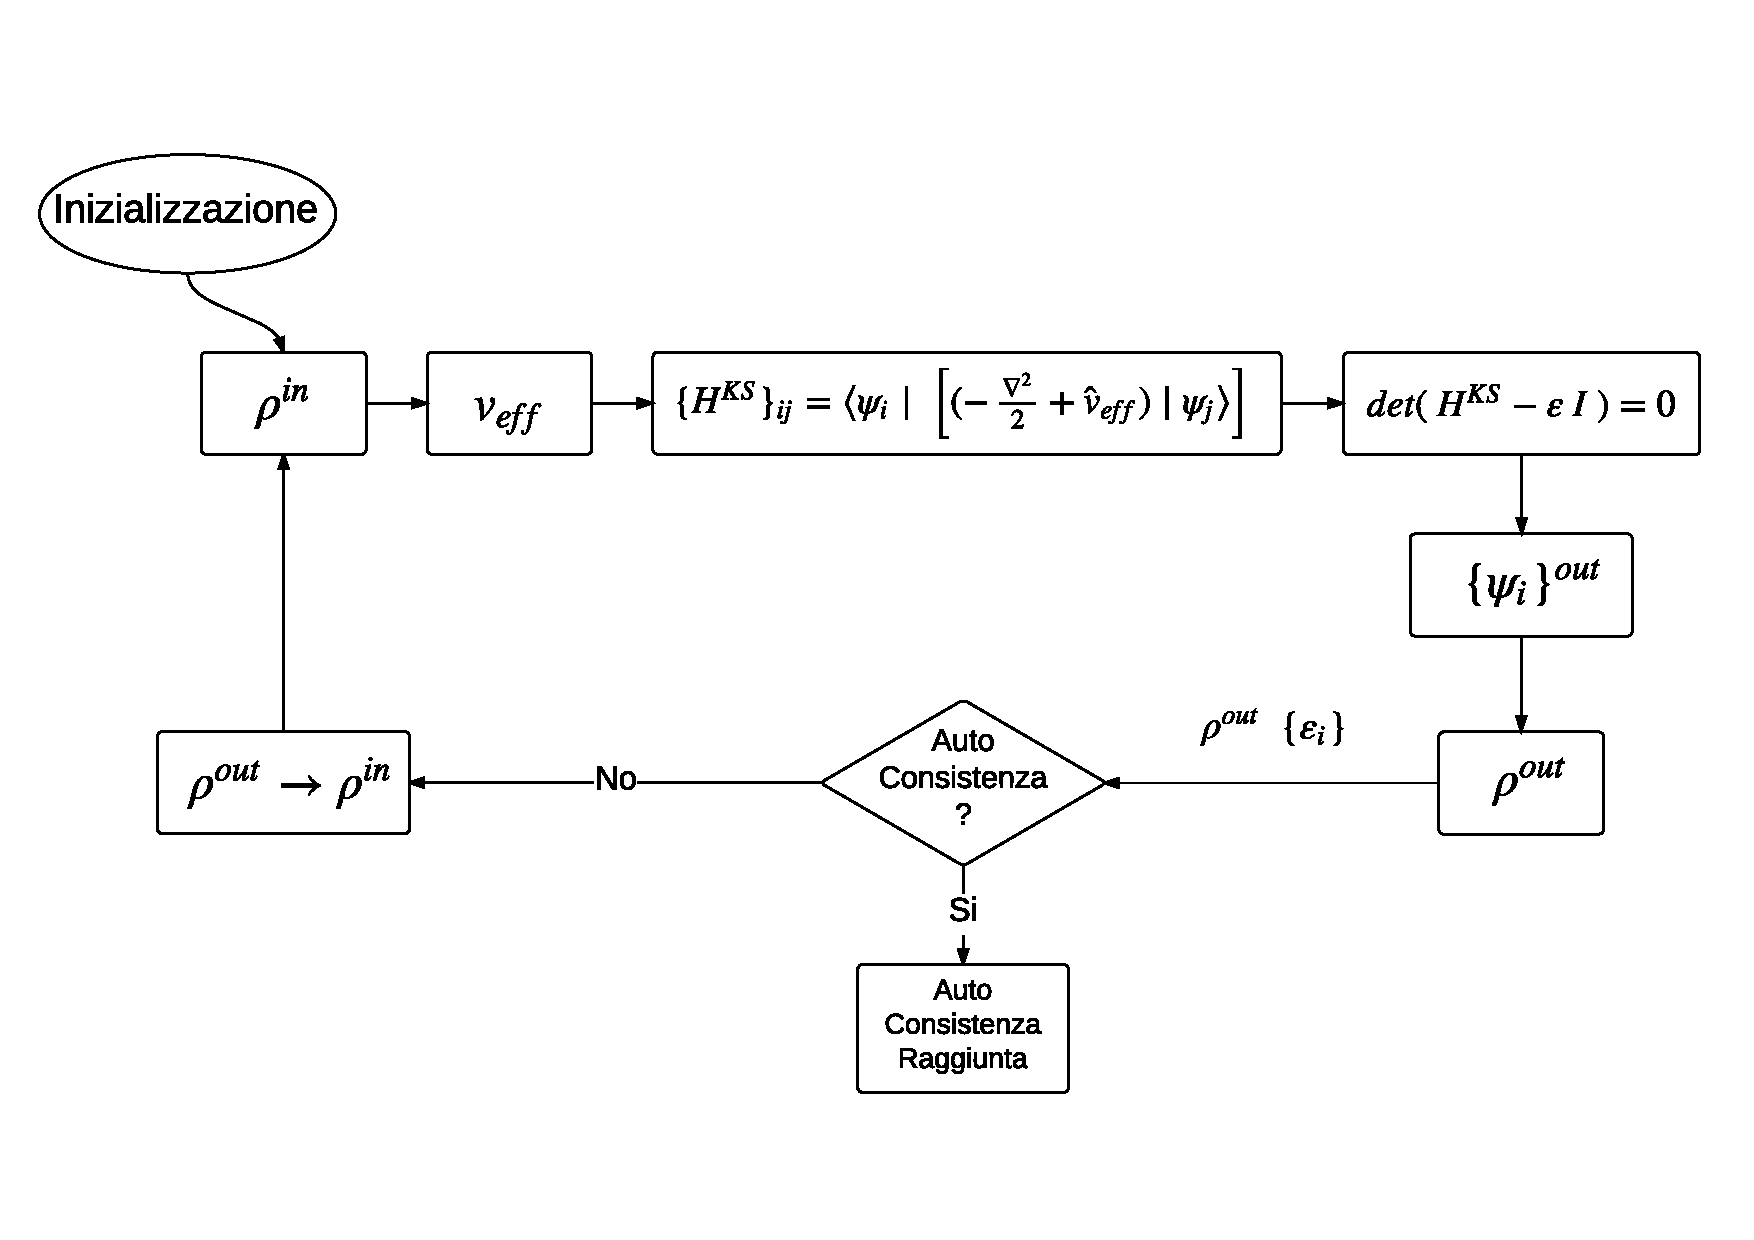
\includegraphics[height=\scfPicHeight\textheight, width=\scfPicWidth\textwidth]{beam_SCF_0.pdf}	
				}
				\only<2>{
					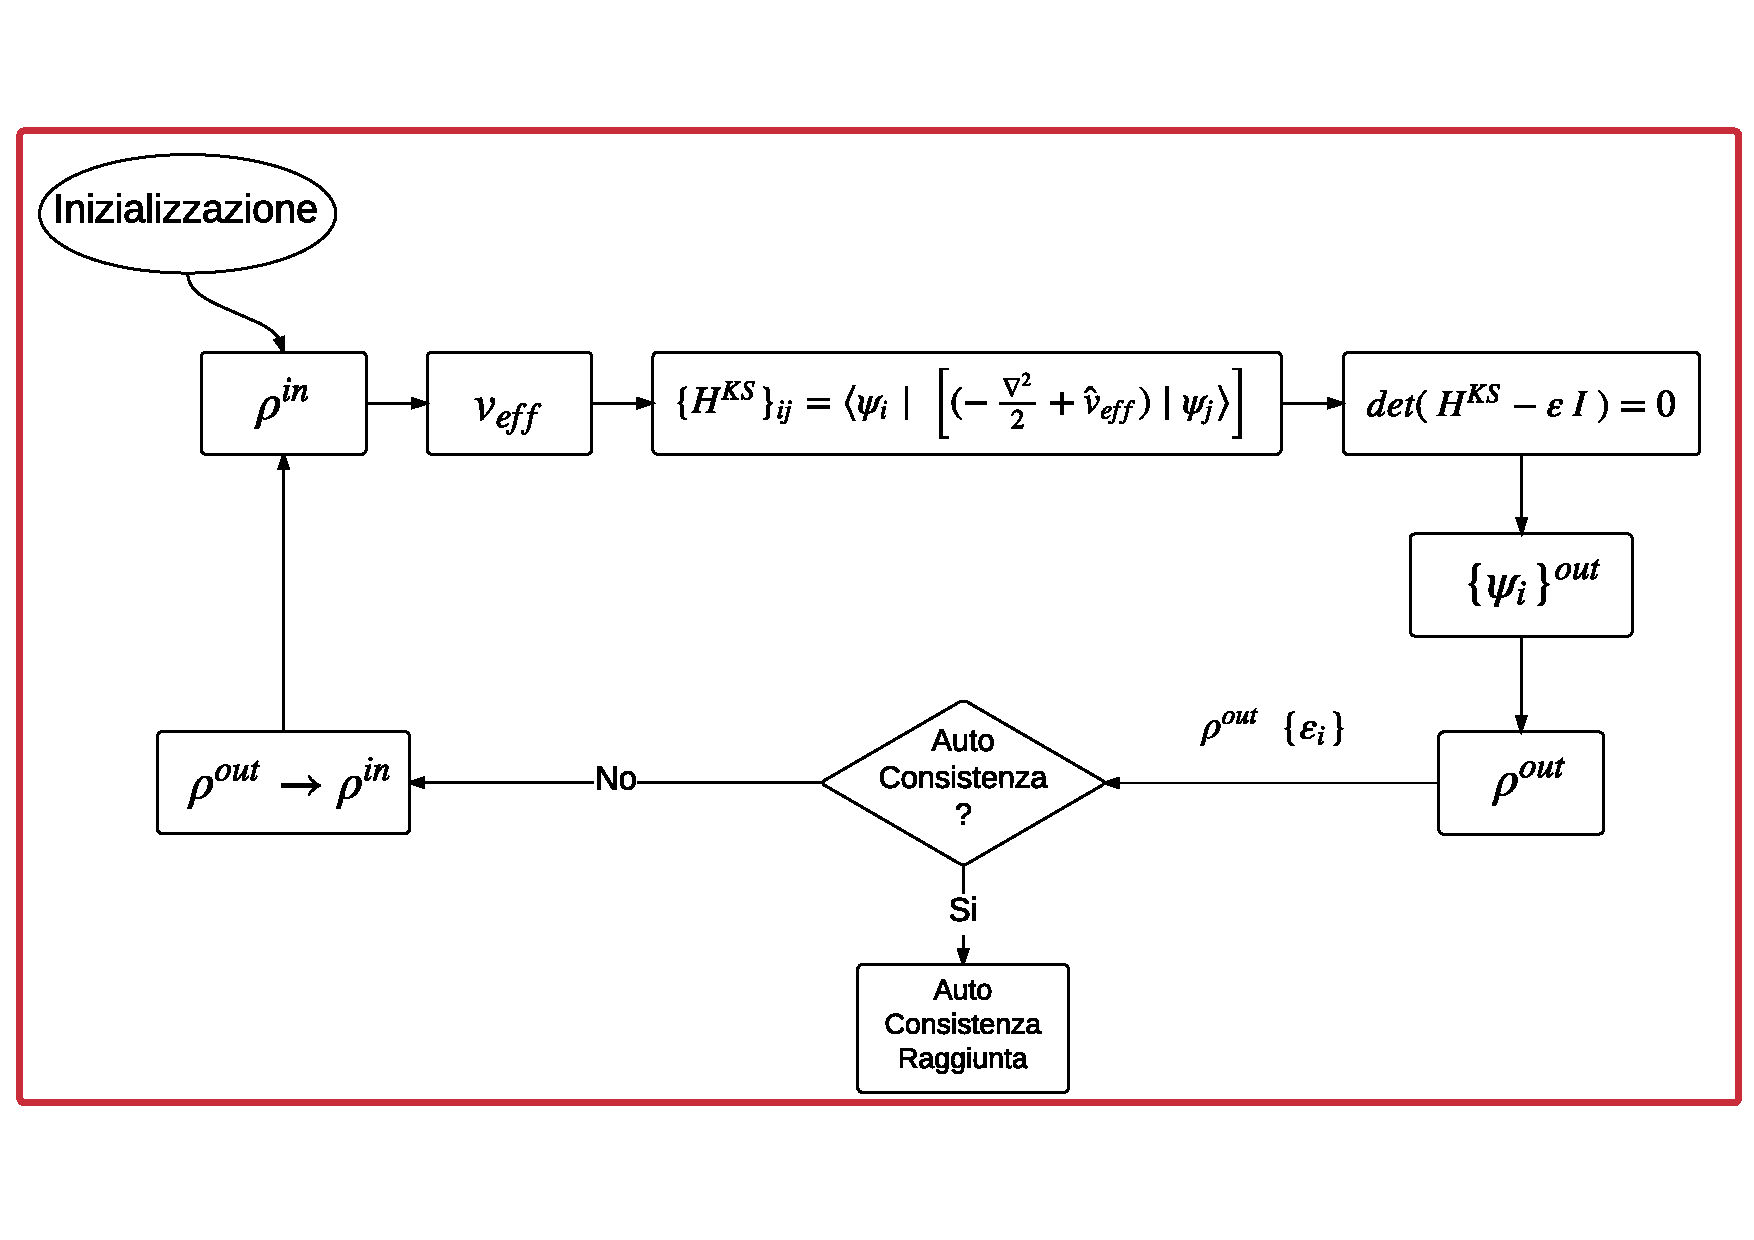
\includegraphics[height=\scfPicHeight\textheight, width=\scfPicWidth\textwidth]{beam_SCF_PWSCF.pdf}	
				}
				\only<\inputPos>{
					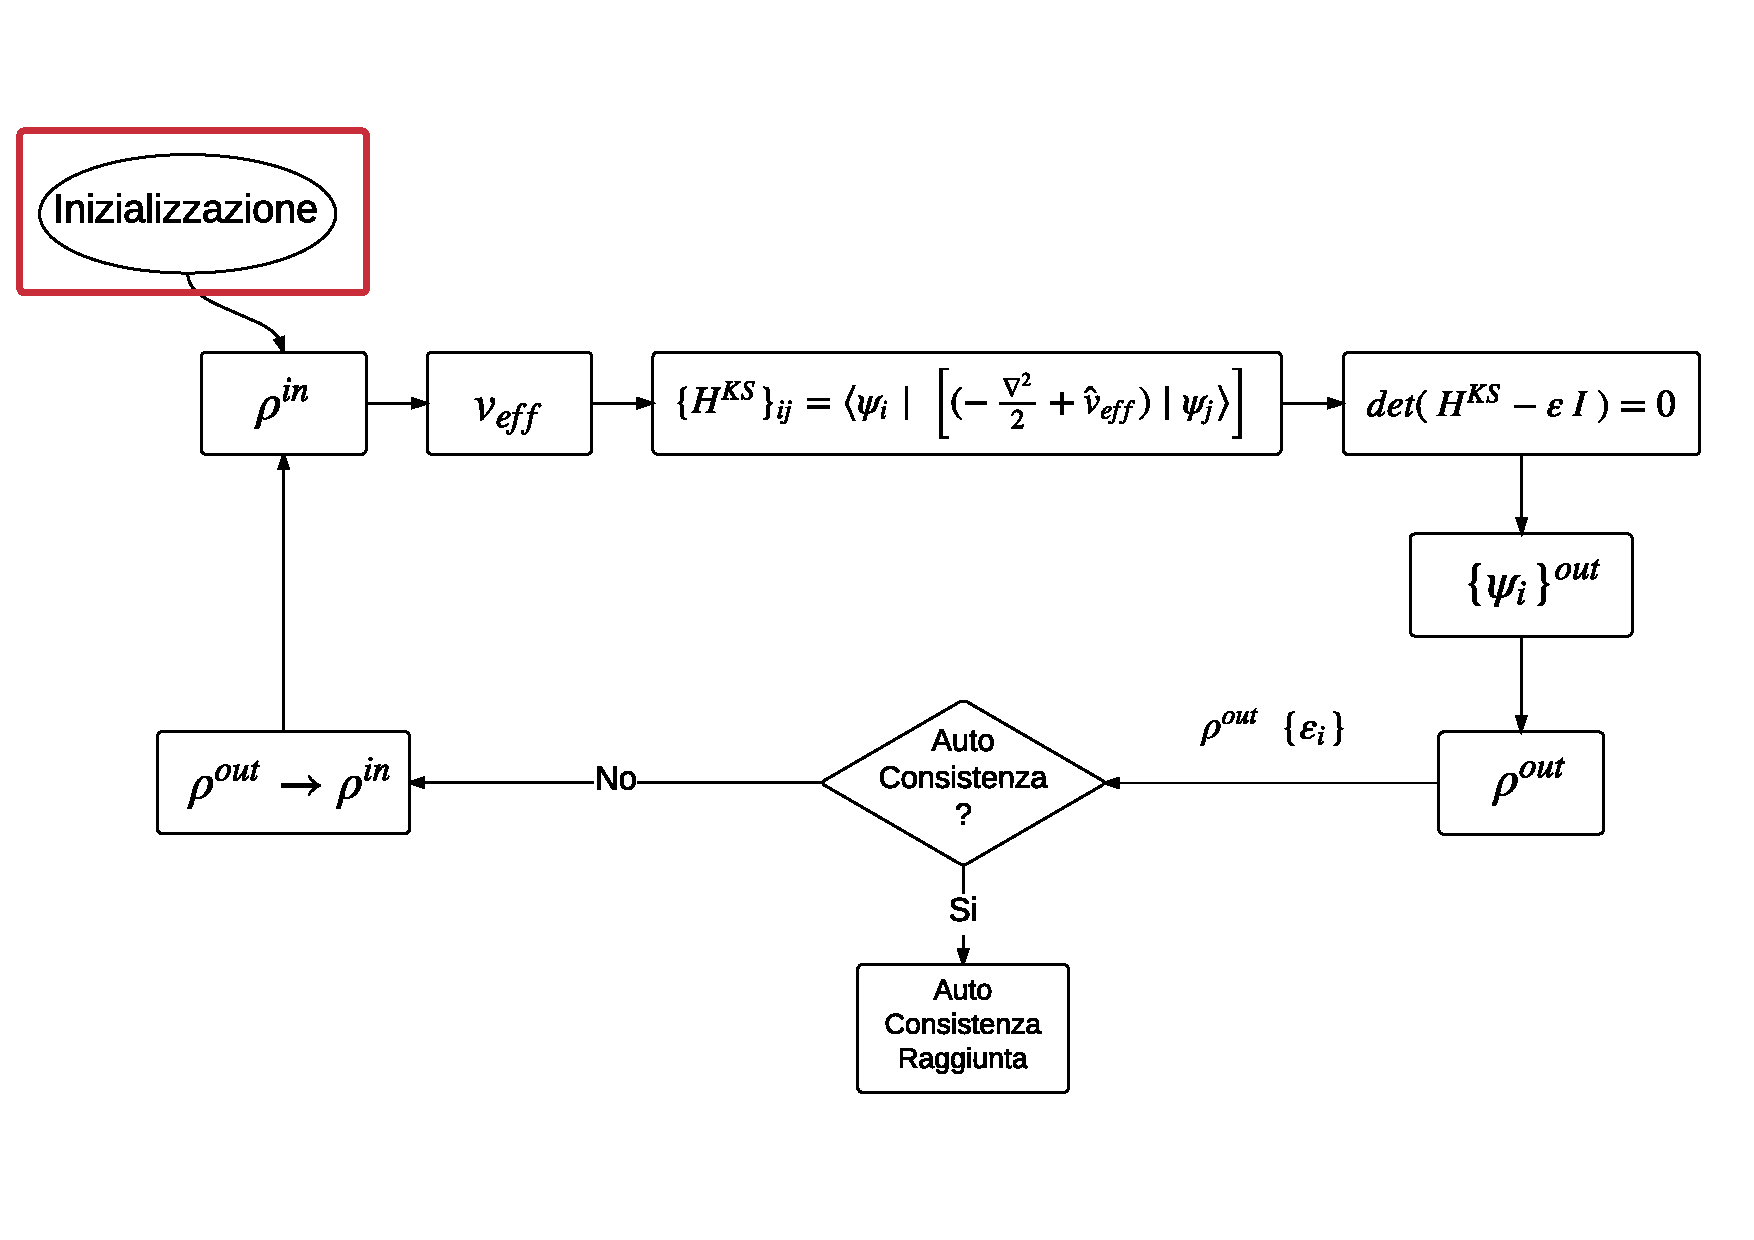
\includegraphics[height=\scfPicHeight\textheight, width=\scfPicWidth\textwidth]{beam_SCF_init_run.pdf}	
				}
				\only<\electronsPos>{
					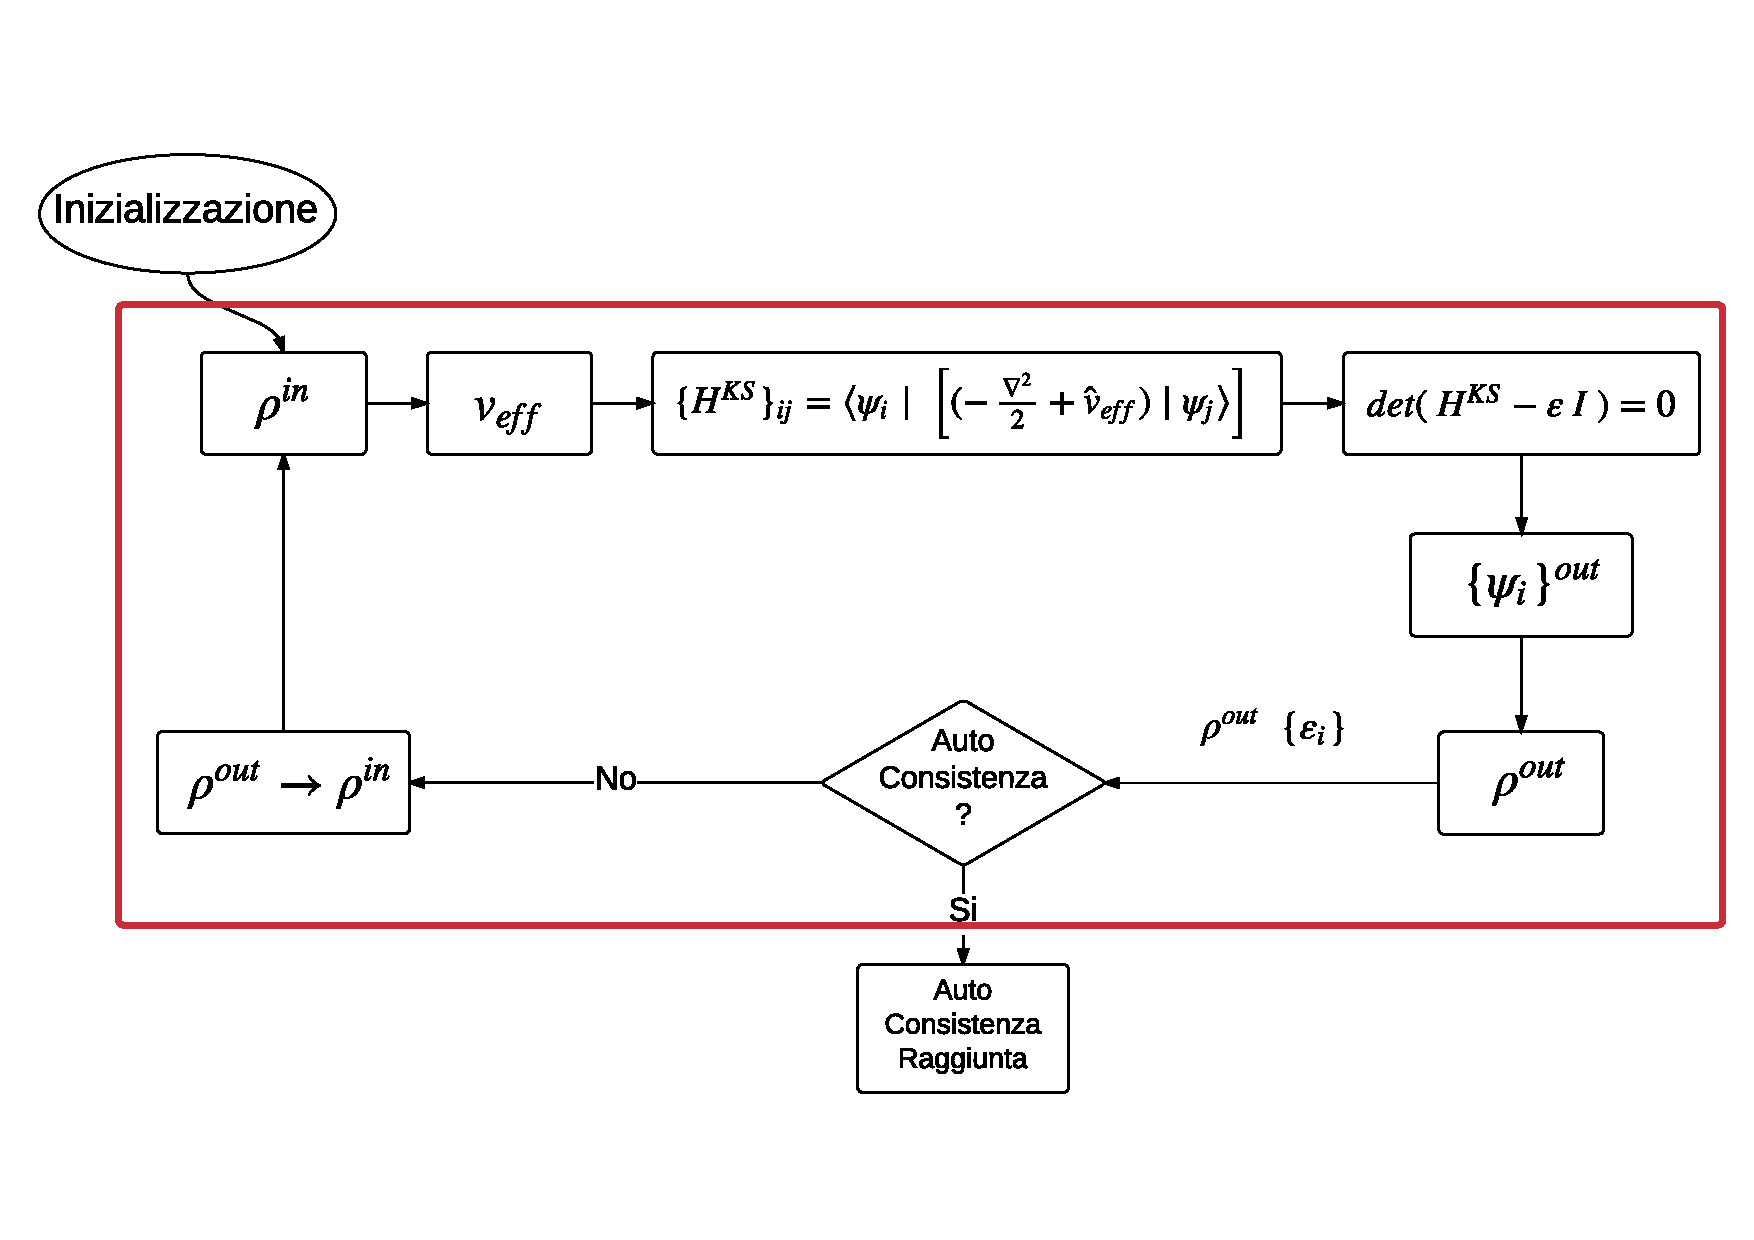
\includegraphics[height=\scfPicHeight\textheight, width=\scfPicWidth\textwidth]{beam_SCF_electrons.pdf}	
				}				
				\only<\cegtergPos>{
					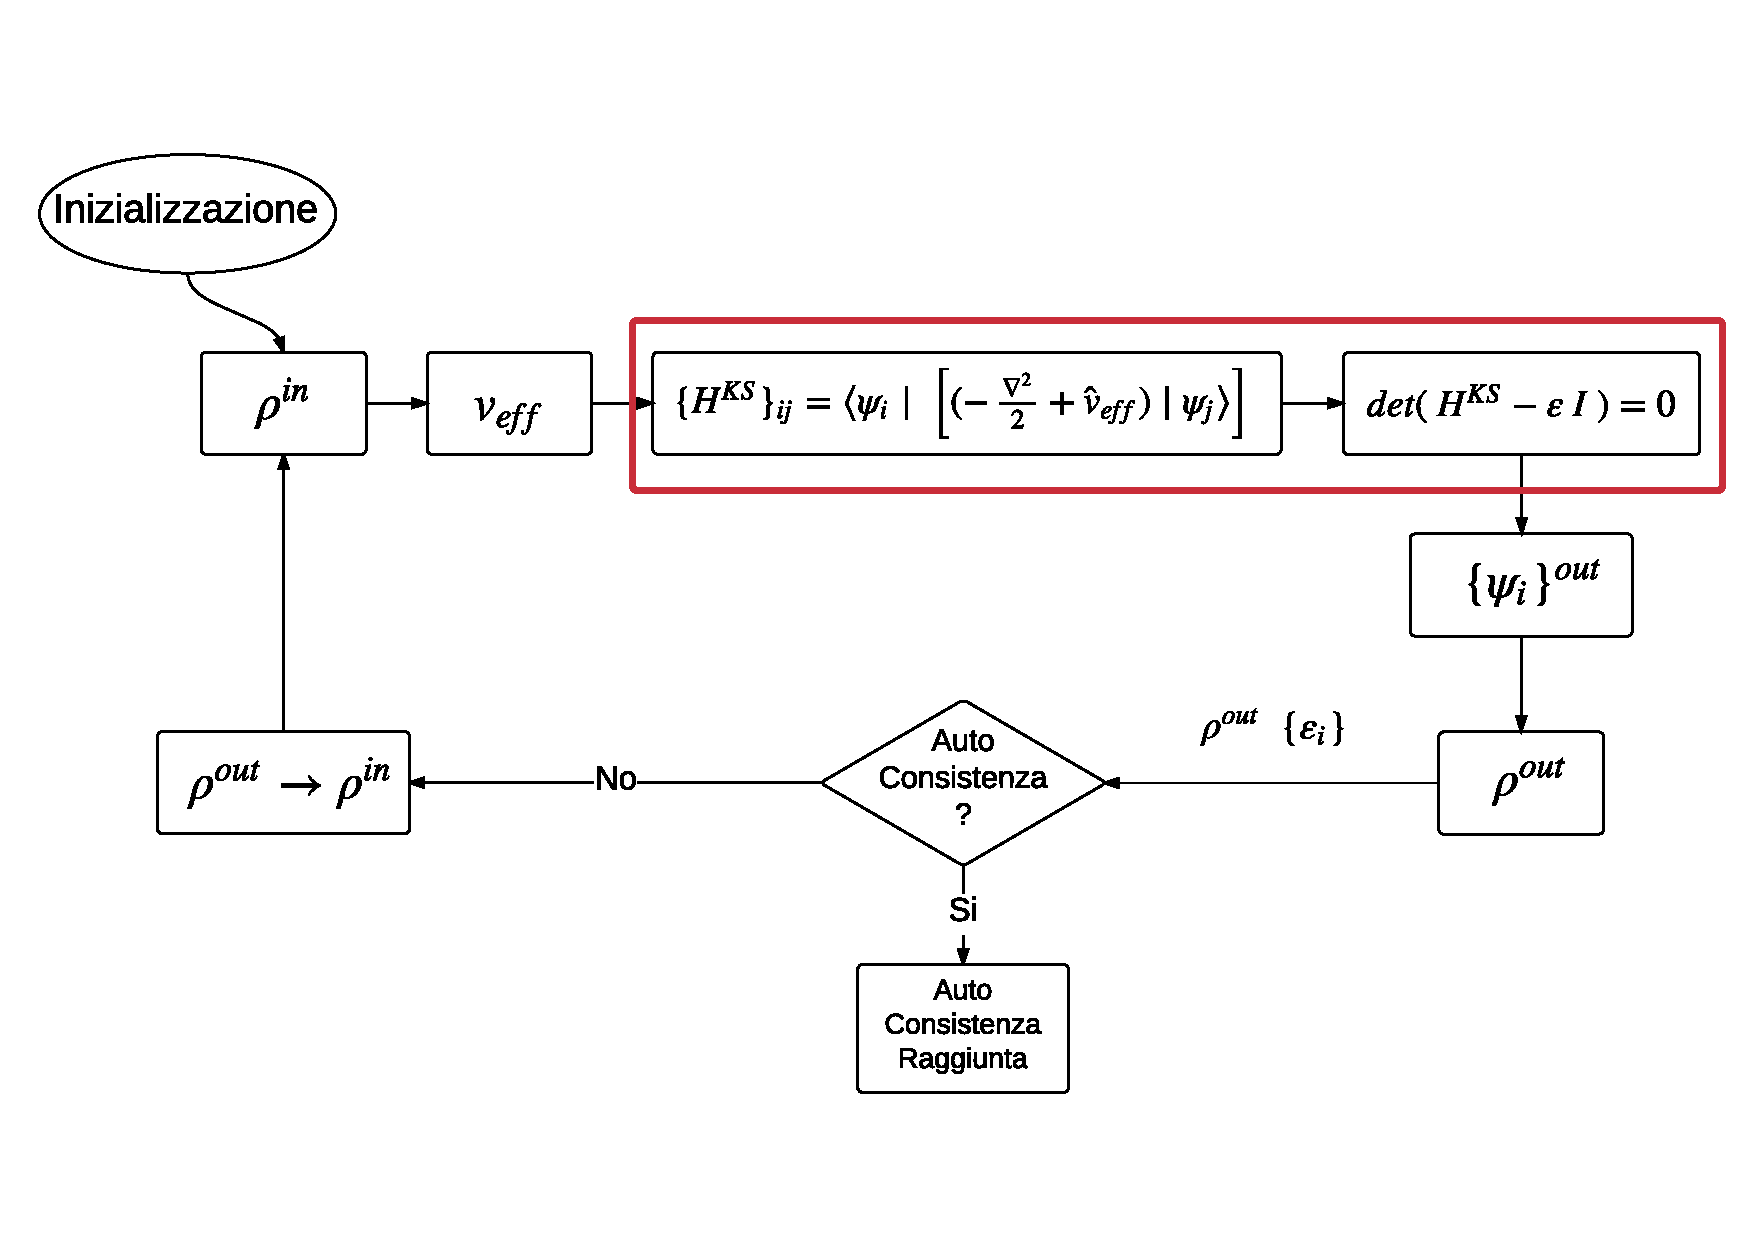
\includegraphics[height=\scfPicHeight\textheight, width=\scfPicWidth\textwidth]{beam_SCF_cegterg.pdf}	
				}
				\only<\hpsiPos>{
					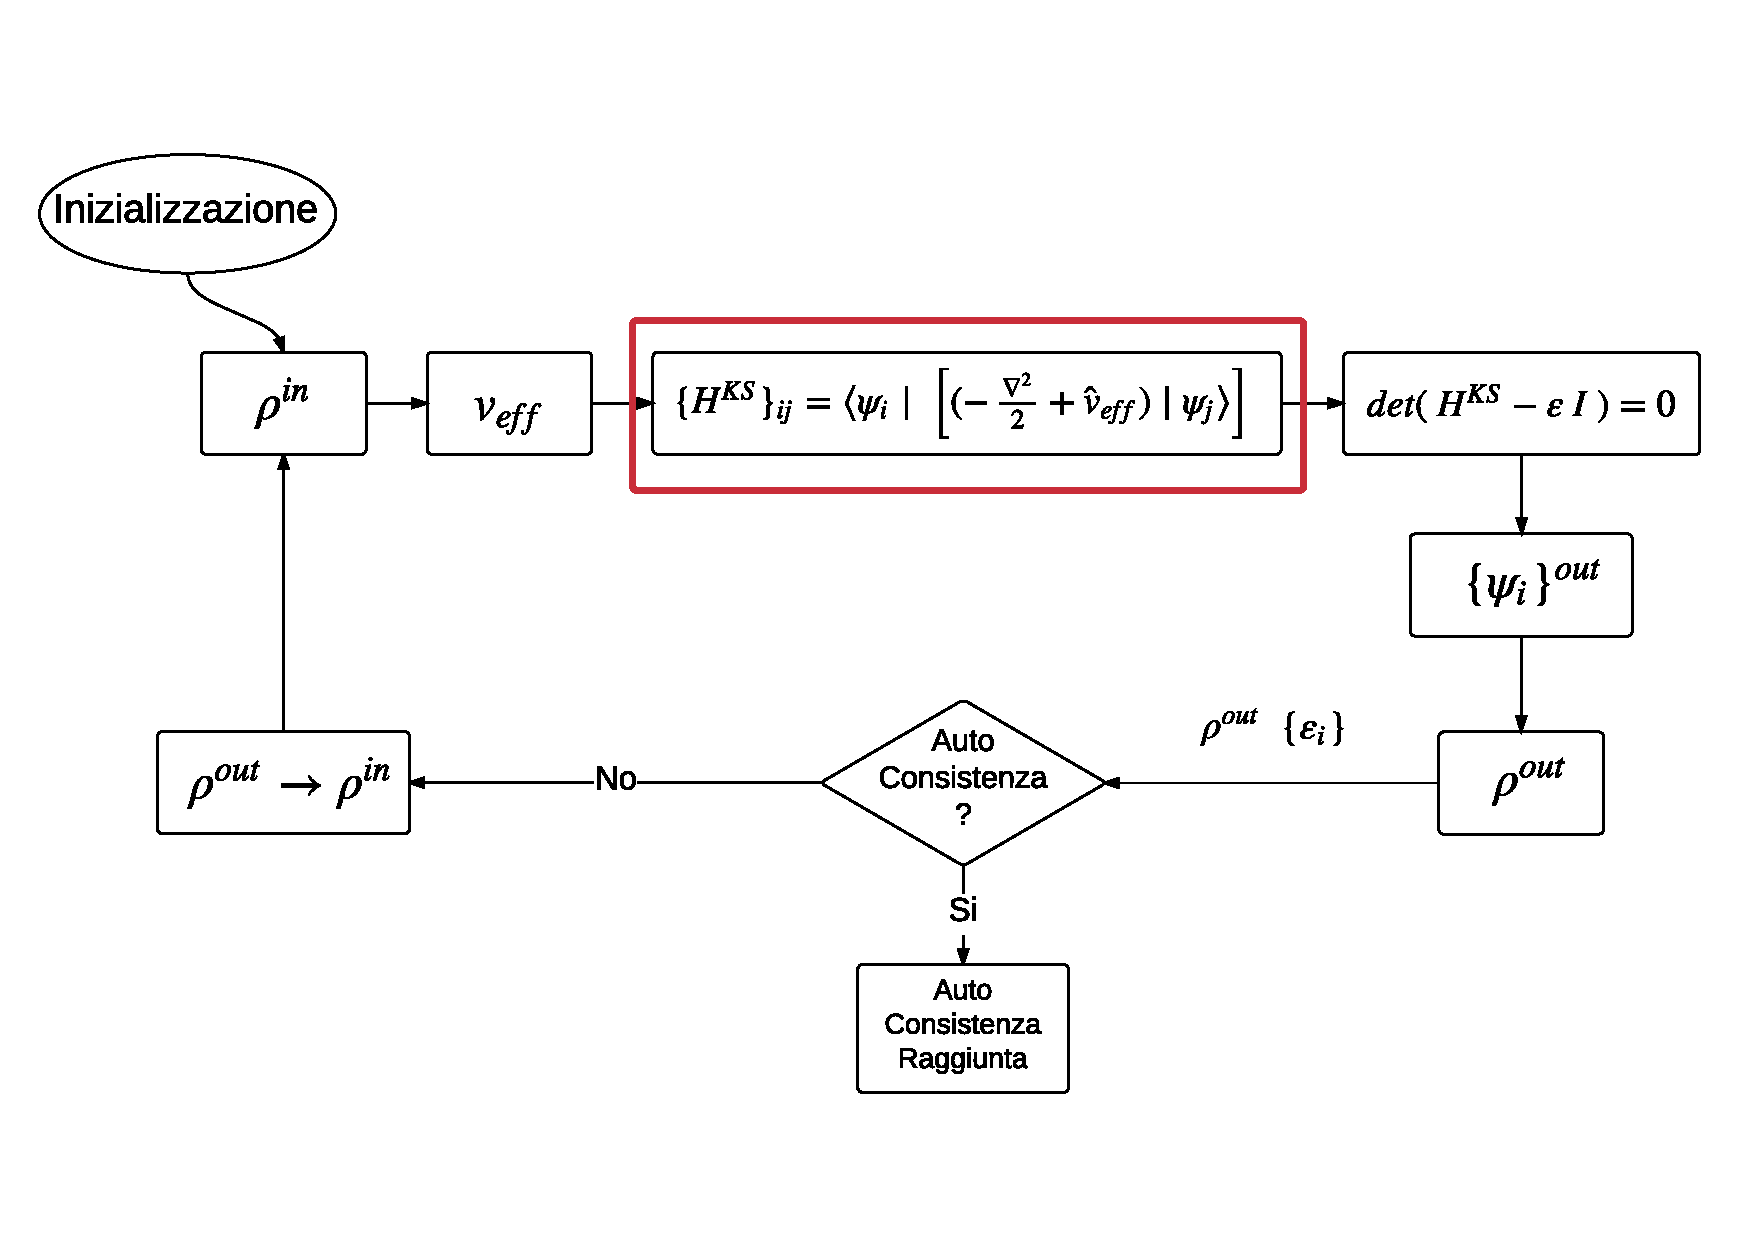
\includegraphics[height=\scfPicHeight\textheight, width=\scfPicWidth\textwidth]{beam_SCF_h_psi.pdf}	
				}
				\only<\cdiaghgPos>{
					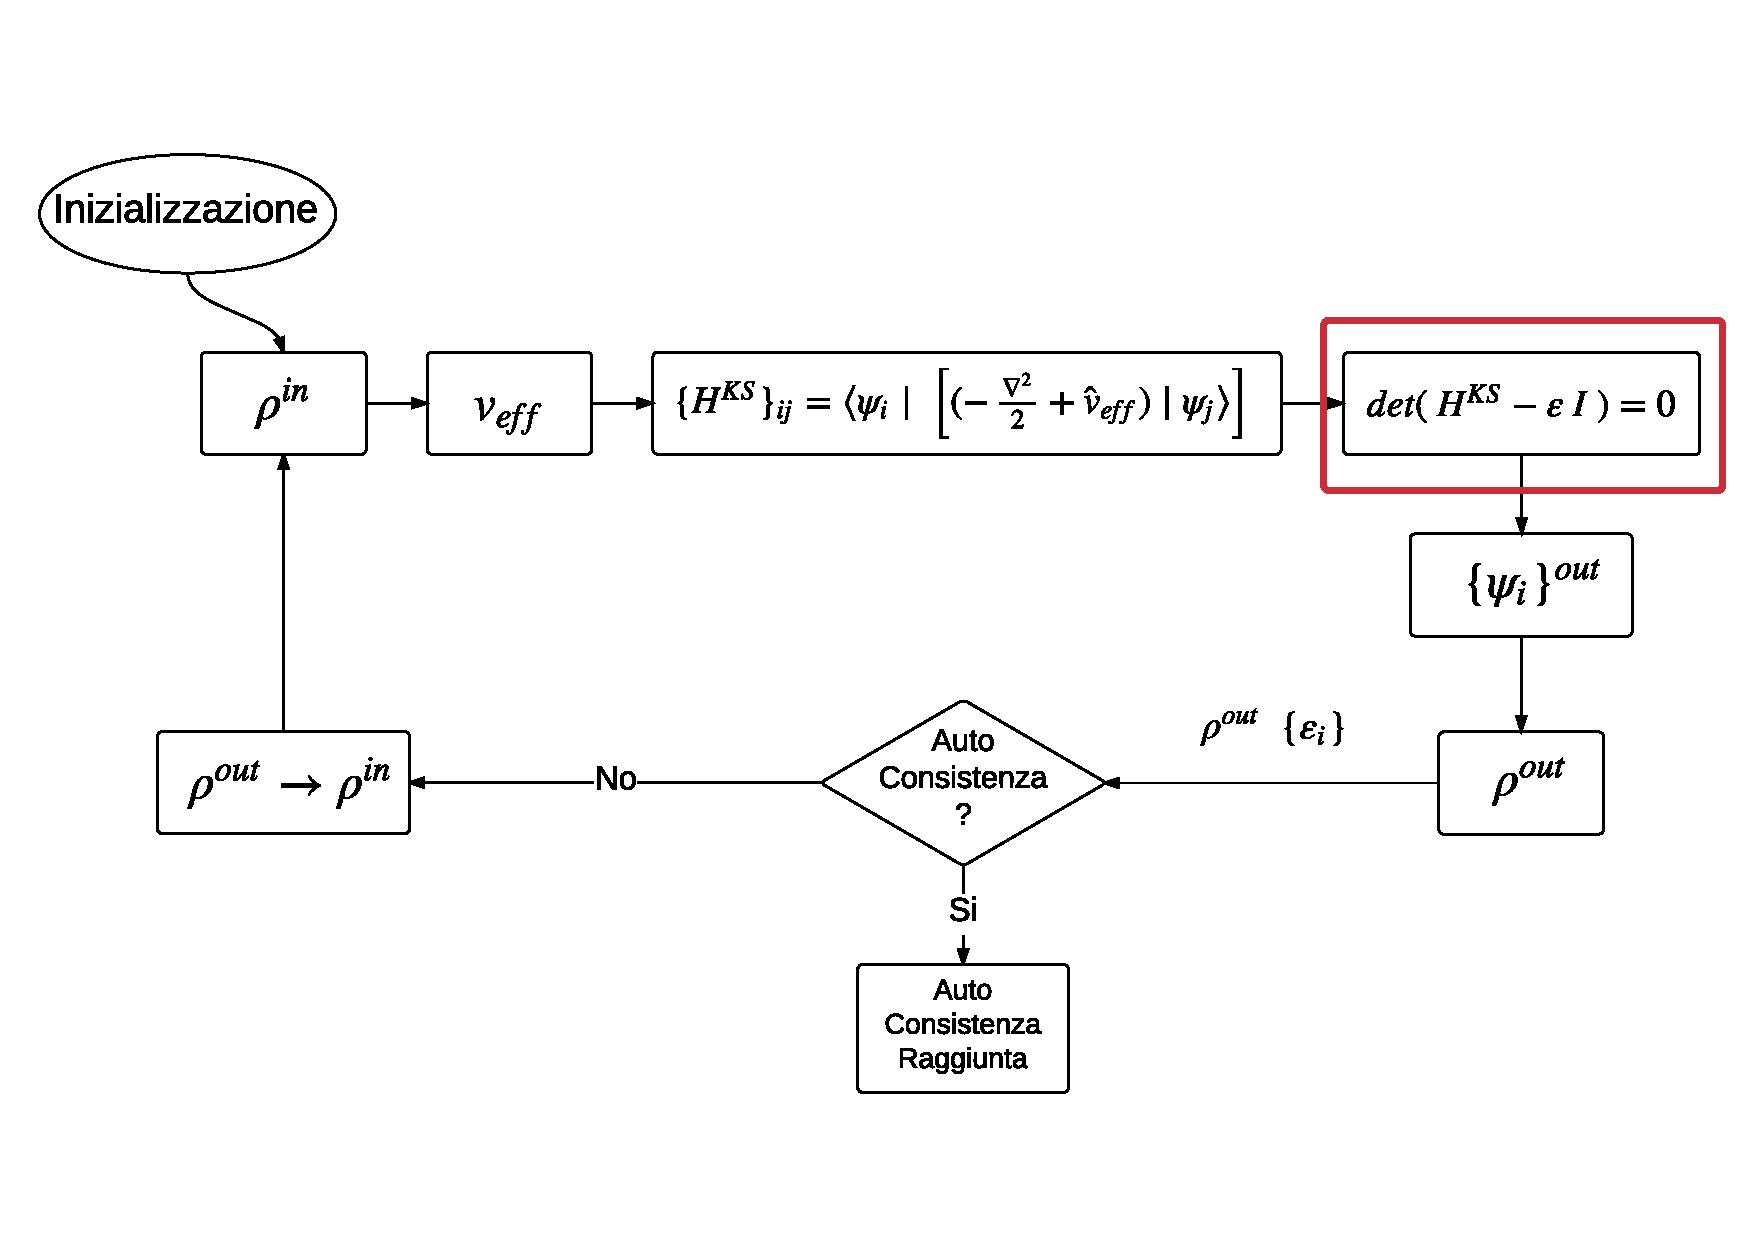
\includegraphics[height=\scfPicHeight\textheight, width=\scfPicWidth\textwidth]{beam_SCF_cdiaghg.pdf}	
				}
				\only<\sumbandPos>{
					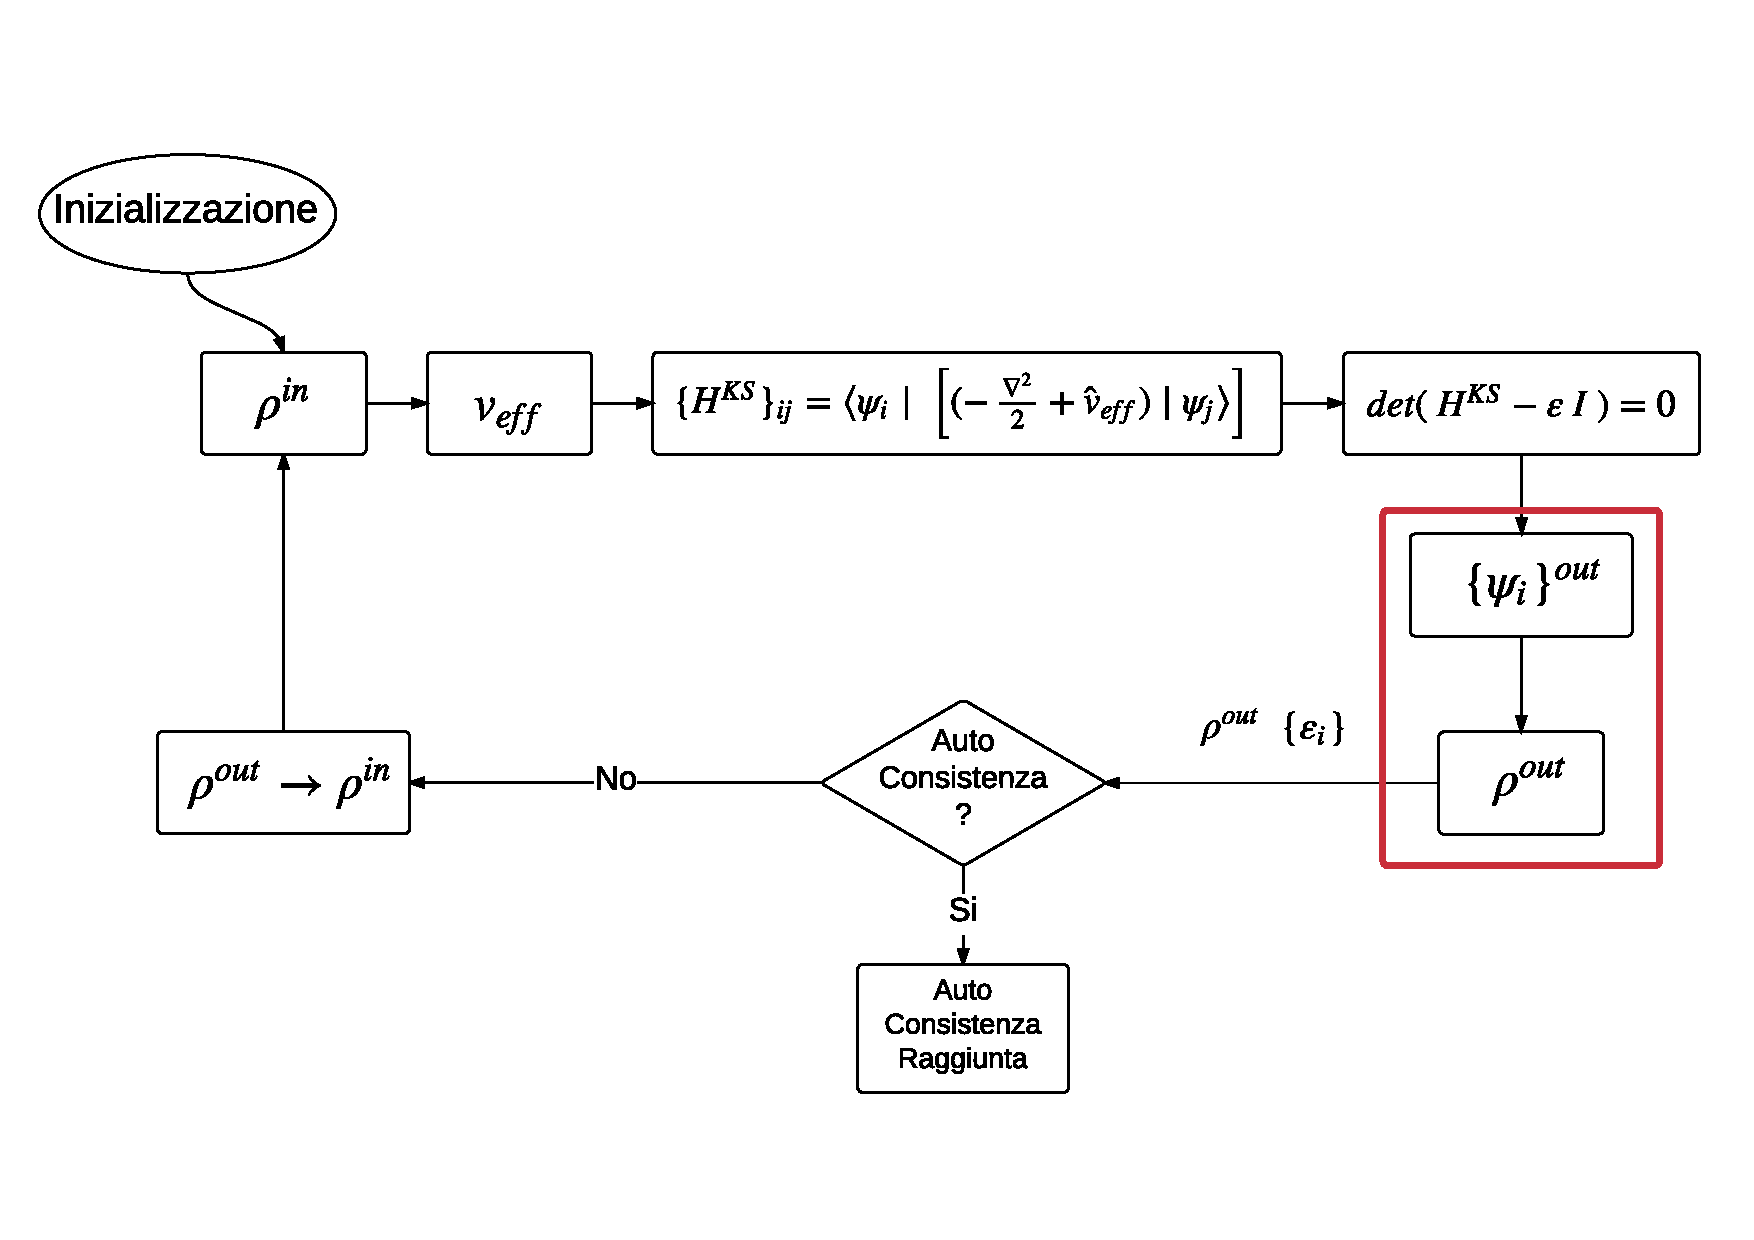
\includegraphics[height=\scfPicHeight\textheight, width=\scfPicWidth\textwidth]{beam_SCF_sum_bands.pdf}	
				}

				\end{flushleft}    	
			\column{0.5\textwidth}

				\only<1->{\vspace{-2cm}}
				
				\only<1,2>{

					\begin{block}{Pacchetto PWscf} 
						\begin{itemize}
							\item Self Consistent DFT
							\item Onde Piane come \textit{basis-set}
						\end{itemize}
					\end{block}
				}
				
				\only<\inputPos>{
					\begin{block}{Inizializzazione} 
						\begin{itemize}
							\item calcolo $\dens$ iniziale
							\item calcolo primi autovettori
							\item calcolo energia iniziale
					\end{itemize}
					\end{block}
				}
				
				\only<\electronsPos>{
					\begin{block}{Problema elettronico} 
						\begin{itemize}
							\item Intero ciclo SCF
							\item Al termine si ottiene $\dens$ di ground state
					\end{itemize}
					\end{block}
				}
				\only<\cegtergPos>{
					\begin{block}{Bande elettroniche} 
						\begin{itemize}
							\item Risoluzione equazioni di Kohn-Sham\\in forma matriciale
					\end{itemize}
					\end{block}
				}
				\only<\hpsiPos>{
					\begin{block}{Valutazione Hamiltoniana} 
						\begin{itemize}
							\item Applicazione laplaciano in spazio reciproco
							\item Applicazione del potenziale in spazio reale
						\end{itemize}
					\end{block}
				}
				\only<\cdiaghgPos>{
					\begin{block}{Diagonalizzazione Hamiltoniana} 
						\begin{itemize}
							\item Algoritmo iterativo di Davidson
						\end{itemize}
					\end{block}
				}
				\only<\sumbandPos>{
					\begin{block}{Calcolo densit\`a elettronica} 
						\begin{itemize}
							\item calcolo occupazione orbitali
							\item $\displaystyle \dens = \sum_{i} f_{\psi_{i}} ~ \psi_{i}^{*KS}(\erre) ~ \psi_{i}^{KS}(\erre)$
						\end{itemize}
					\end{block}
				}
				\only<\fftPos,\fftscatterPos>{
					\begin{block}{Moduli generici} 
						\begin{itemize}
							\visible<\fftPos,\fftscatterPos>{\item Calcolo FFT}
							\visible<\fftscatterPos>{\item Distribuzione griglia}

						\end{itemize}
					\end{block}
				}
				
    	\end{columns}

    \end{minipage}

    \nointerlineskip
    \begin{minipage}[b][0.5\textheight][t]{\textwidth}
        	\begin{columns}
			\column{0.5\textwidth}
				
			\column{0.5\textwidth}
				\vspace{-1cm}
				\begin{center}
			   	\only<1>{
					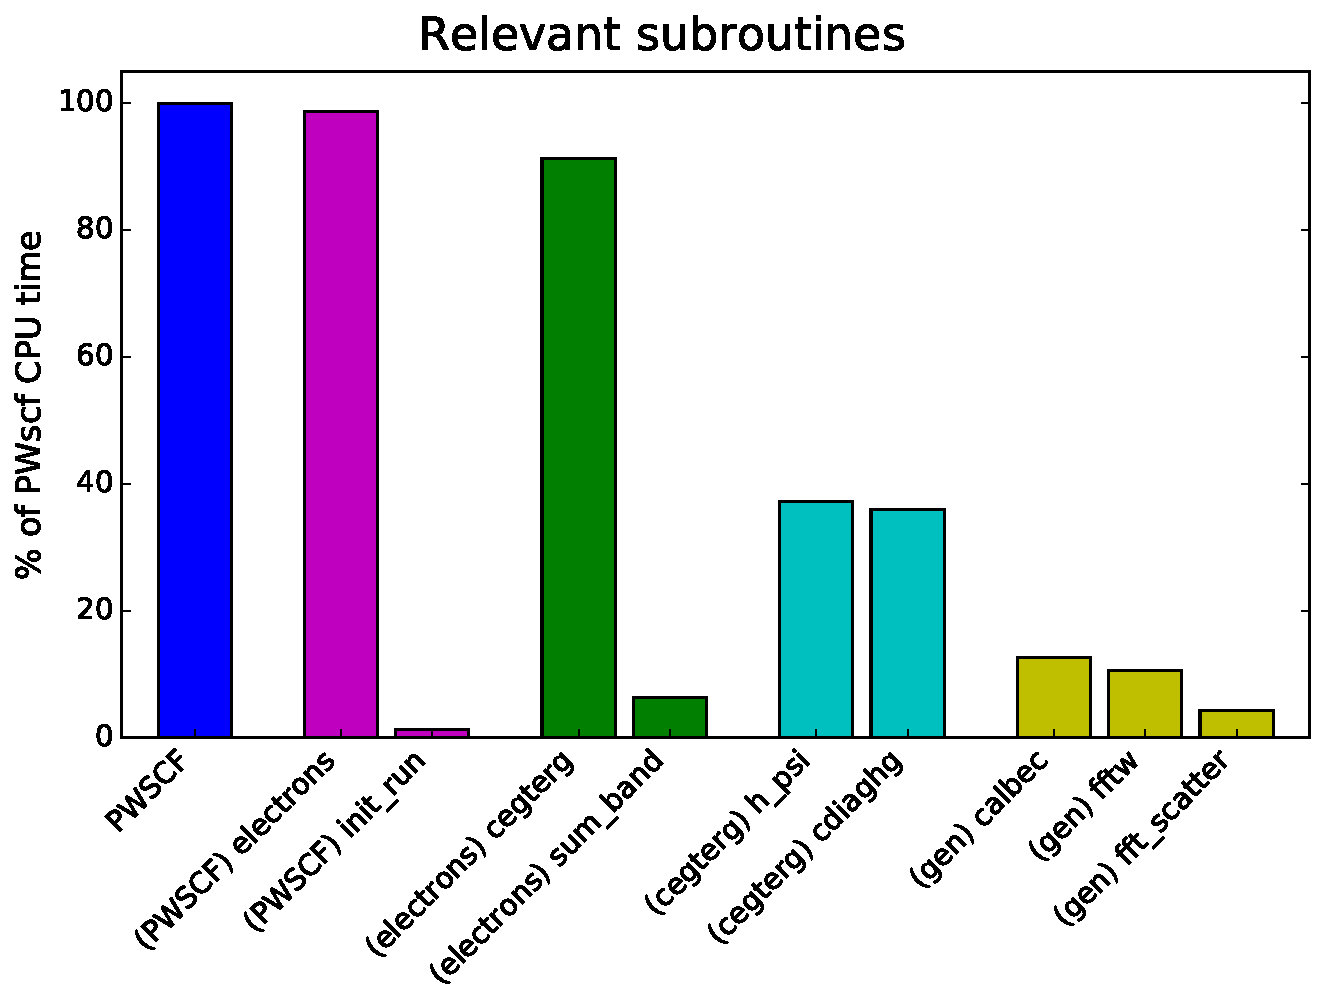
\includegraphics[height=0.5\textheight, width=1\textwidth]{beam_relevant_subroutines.pdf}	
				}
				\only<2>{
					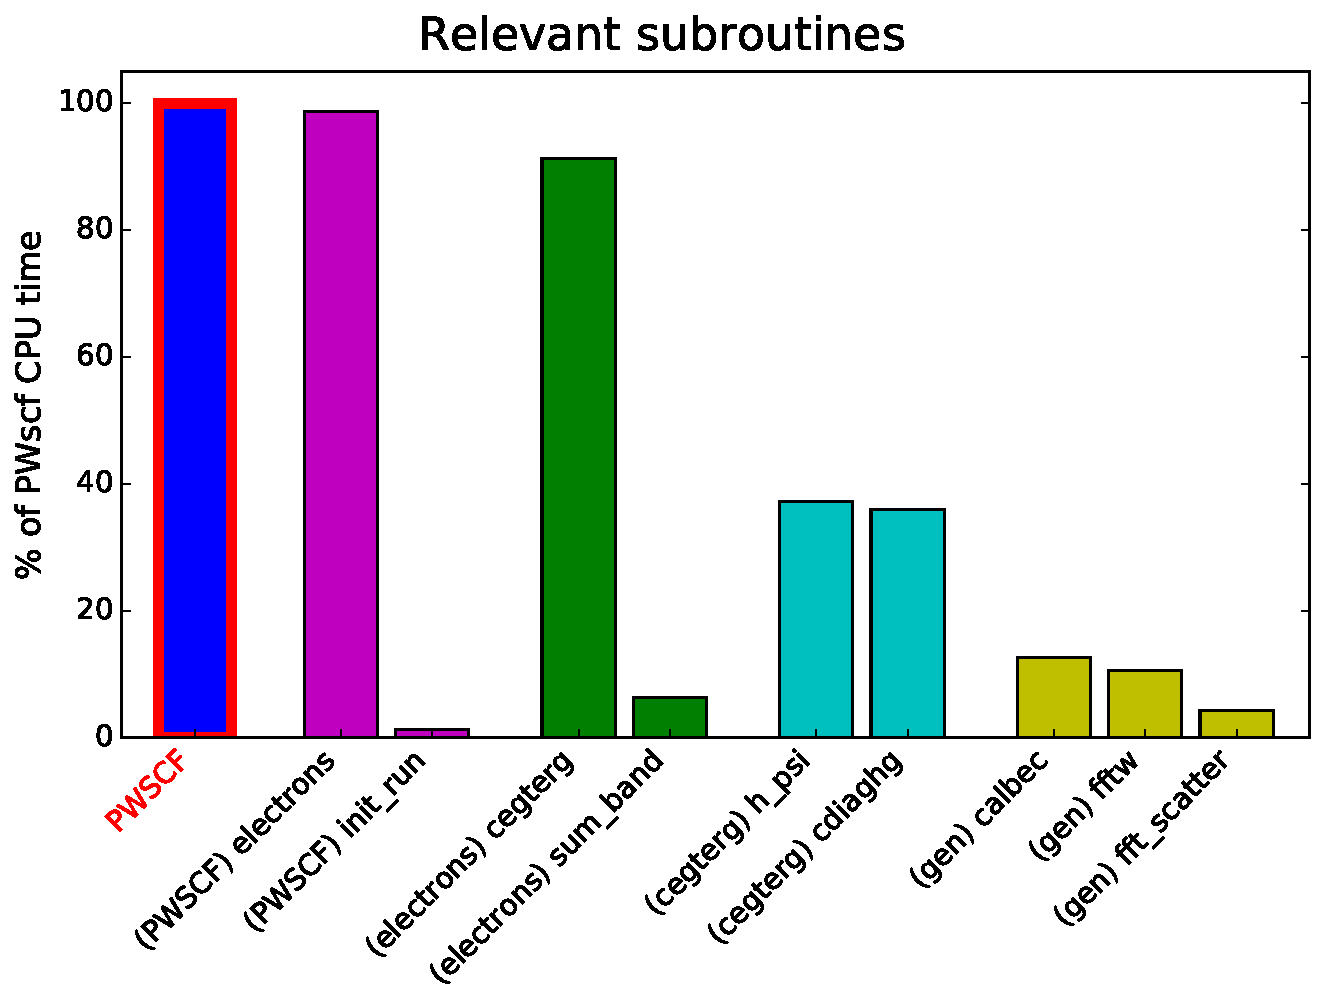
\includegraphics[height=0.5\textheight, width=1\textwidth]{beam_relevant_subroutines_PWSCF.pdf}	
				}
				\only<3>{
					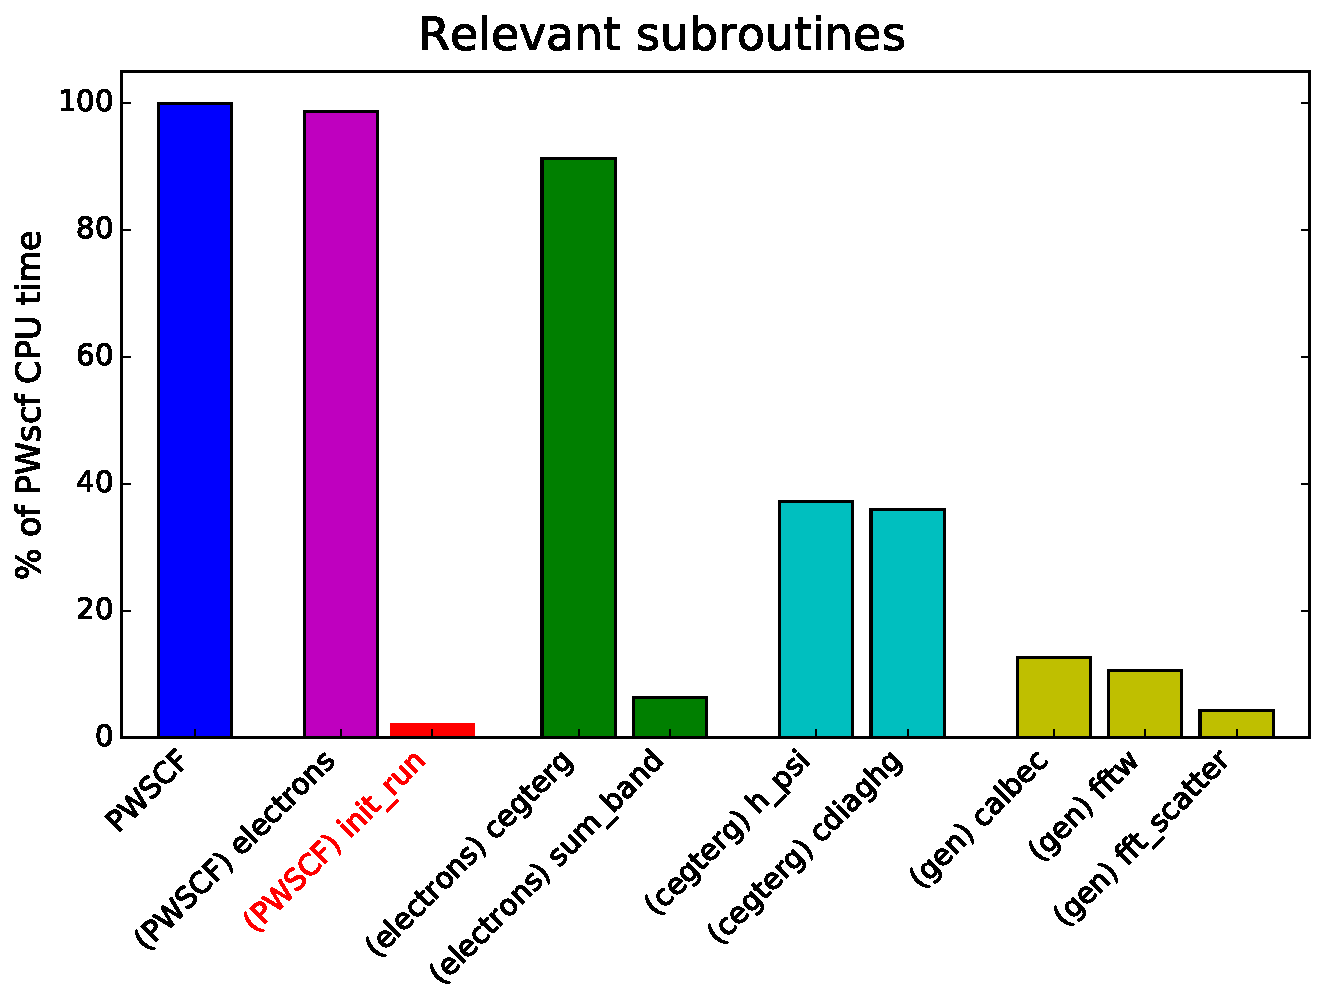
\includegraphics[height=0.5\textheight, width=1\textwidth]{beam_relevant_subroutines_init_run.pdf}	
				}
				\only<4>{
					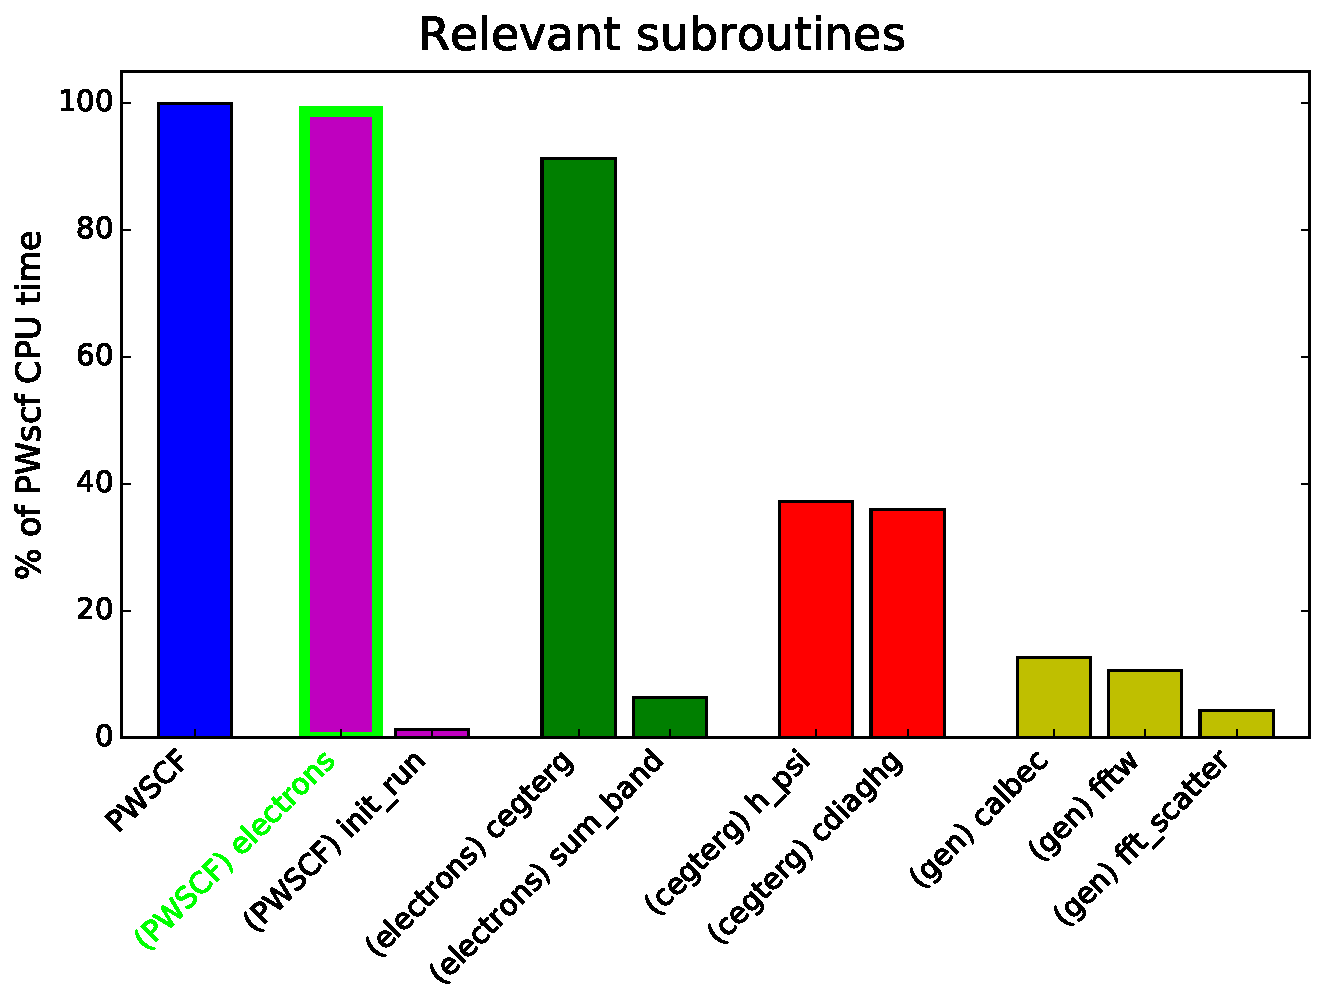
\includegraphics[height=0.5\textheight, width=1\textwidth]{beam_relevant_subroutines_electrons.pdf}	
				}
				\only<5>{
					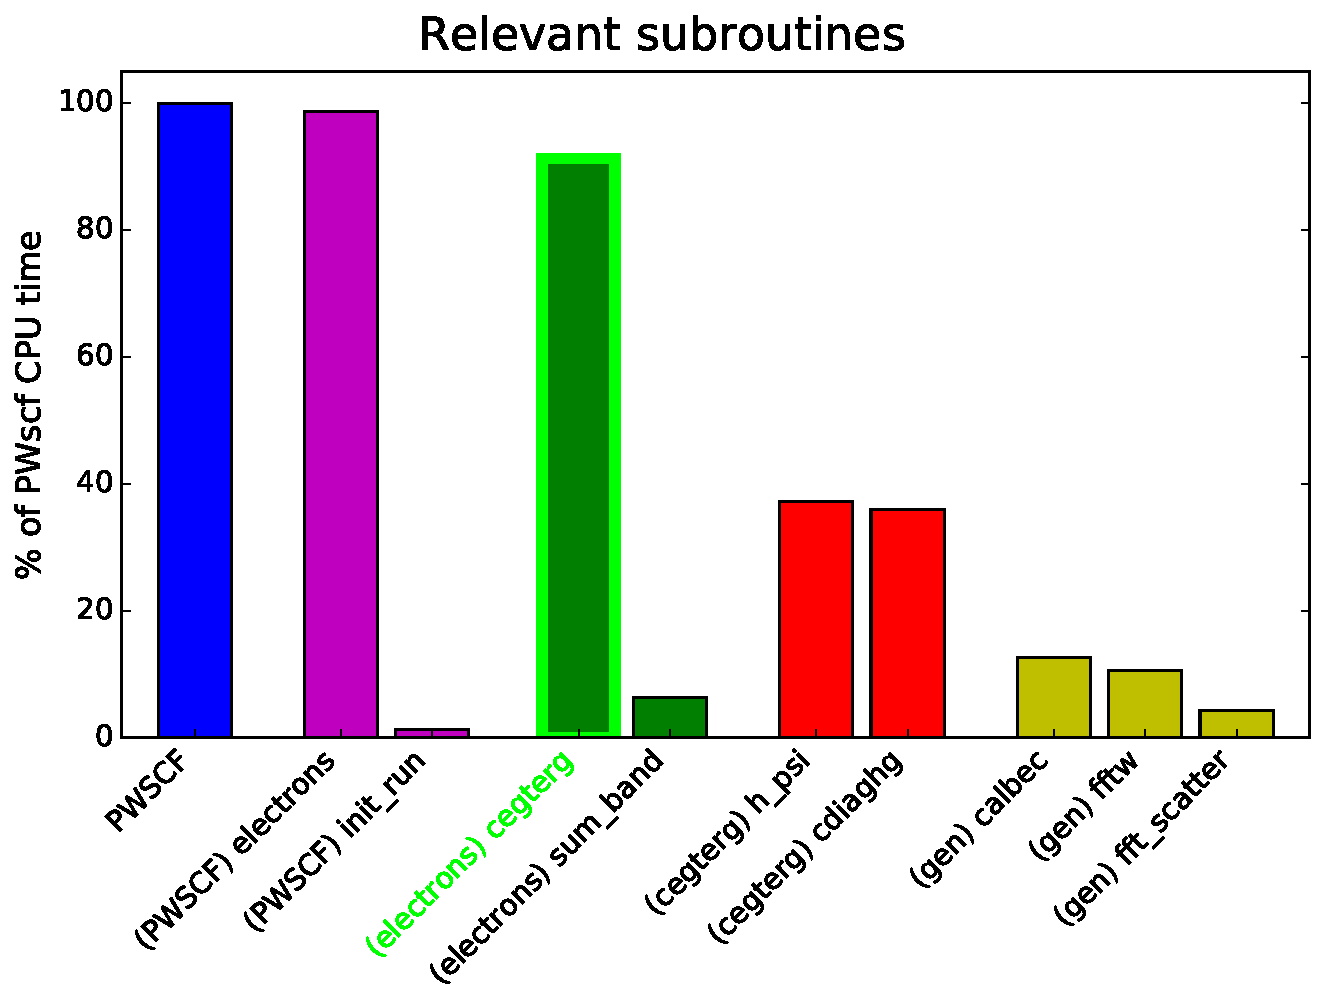
\includegraphics[height=0.5\textheight, width=1\textwidth]{beam_relevant_subroutines_cegterg.pdf}	
				}
				\only<6>{
					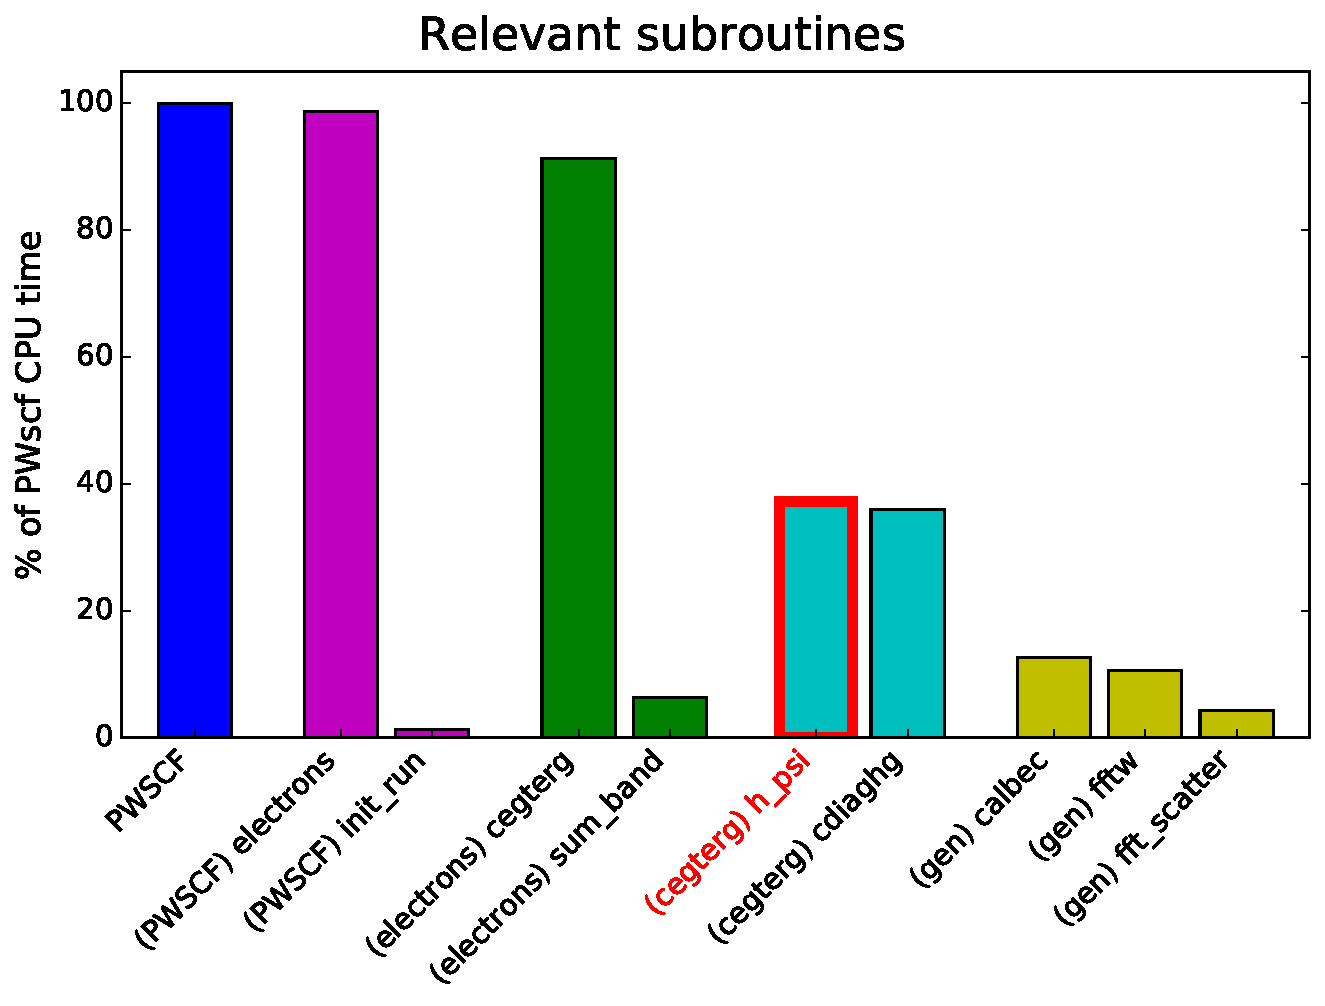
\includegraphics[height=0.5\textheight, width=1\textwidth]{beam_relevant_subroutines_h_psi.pdf}	
				}
				\only<7>{
					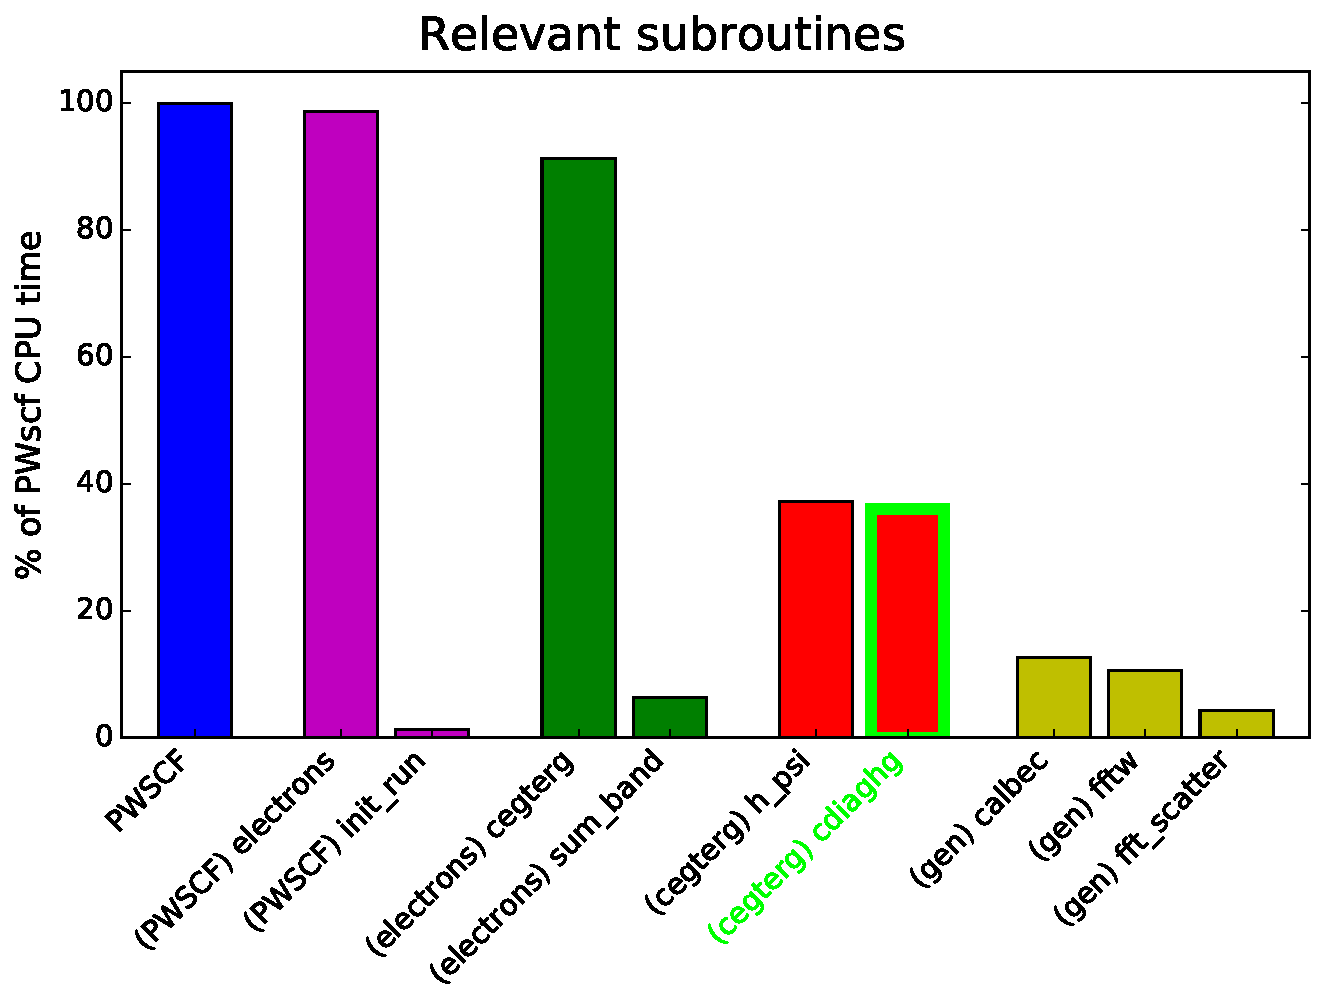
\includegraphics[height=0.5\textheight, width=1\textwidth]{beam_relevant_subroutines_cdiaghg.pdf}	
				}				
				\only<8>{
					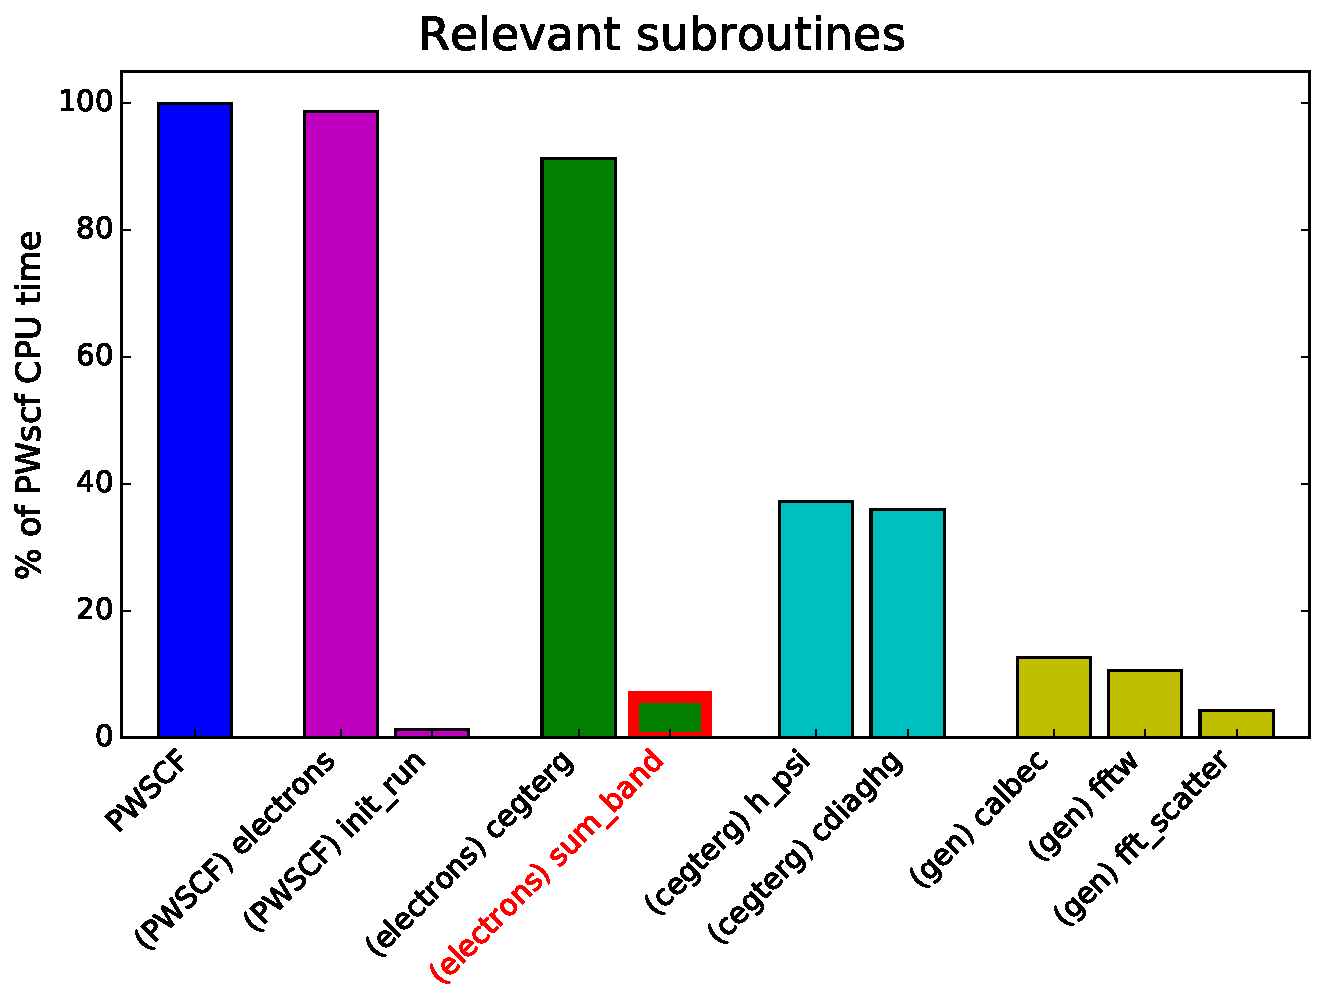
\includegraphics[height=0.5\textheight, width=1\textwidth]{beam_relevant_subroutines_sum_band.pdf}	
				}
				\only<9>{
					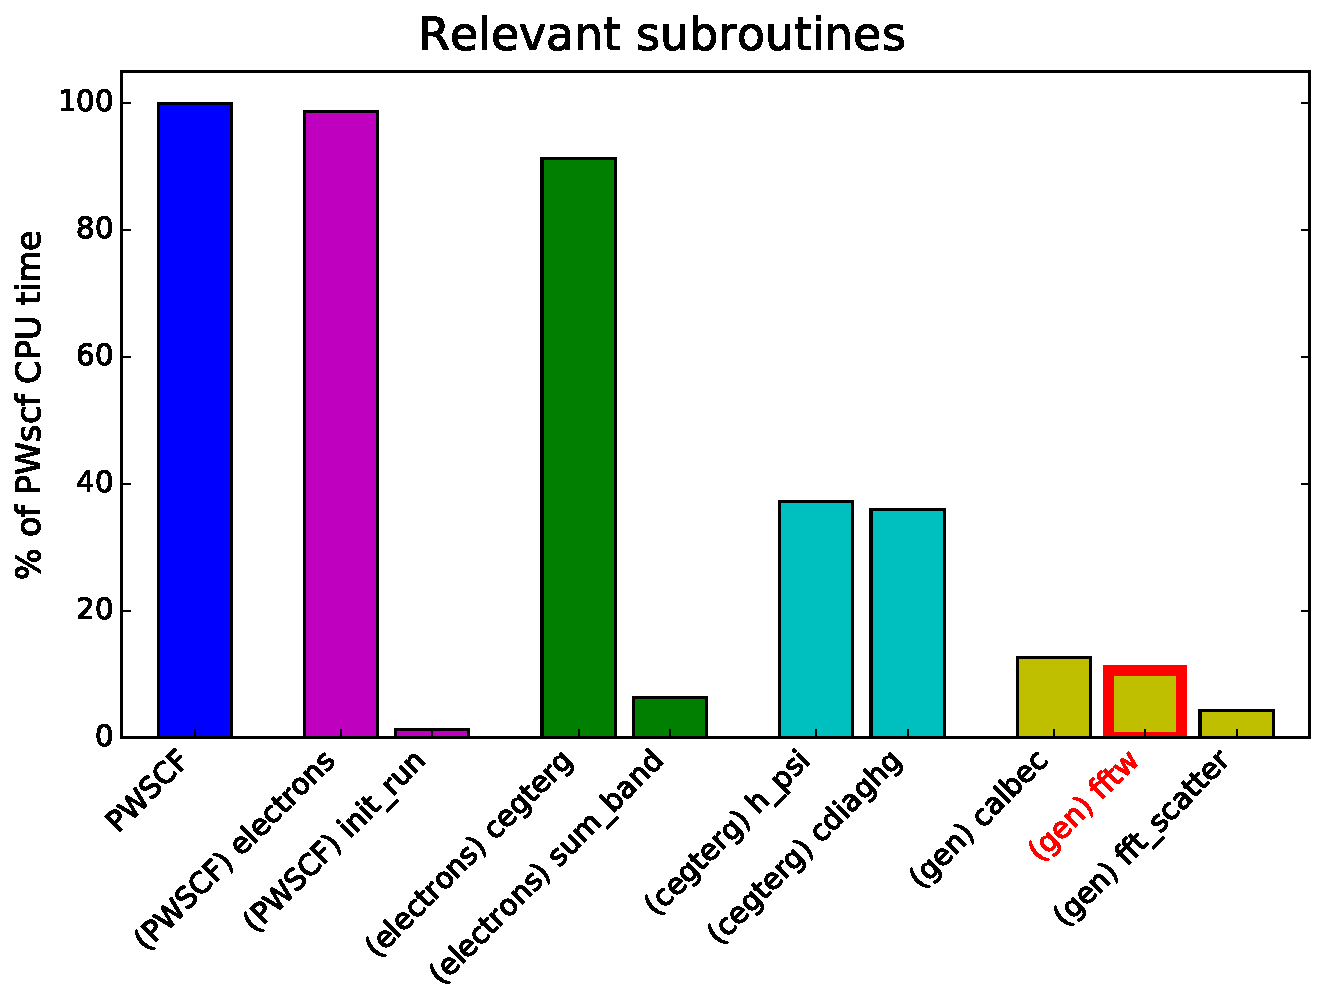
\includegraphics[height=0.5\textheight, width=1\textwidth]{beam_relevant_subroutines_fftw.pdf}	
				}
				\only<10>{
					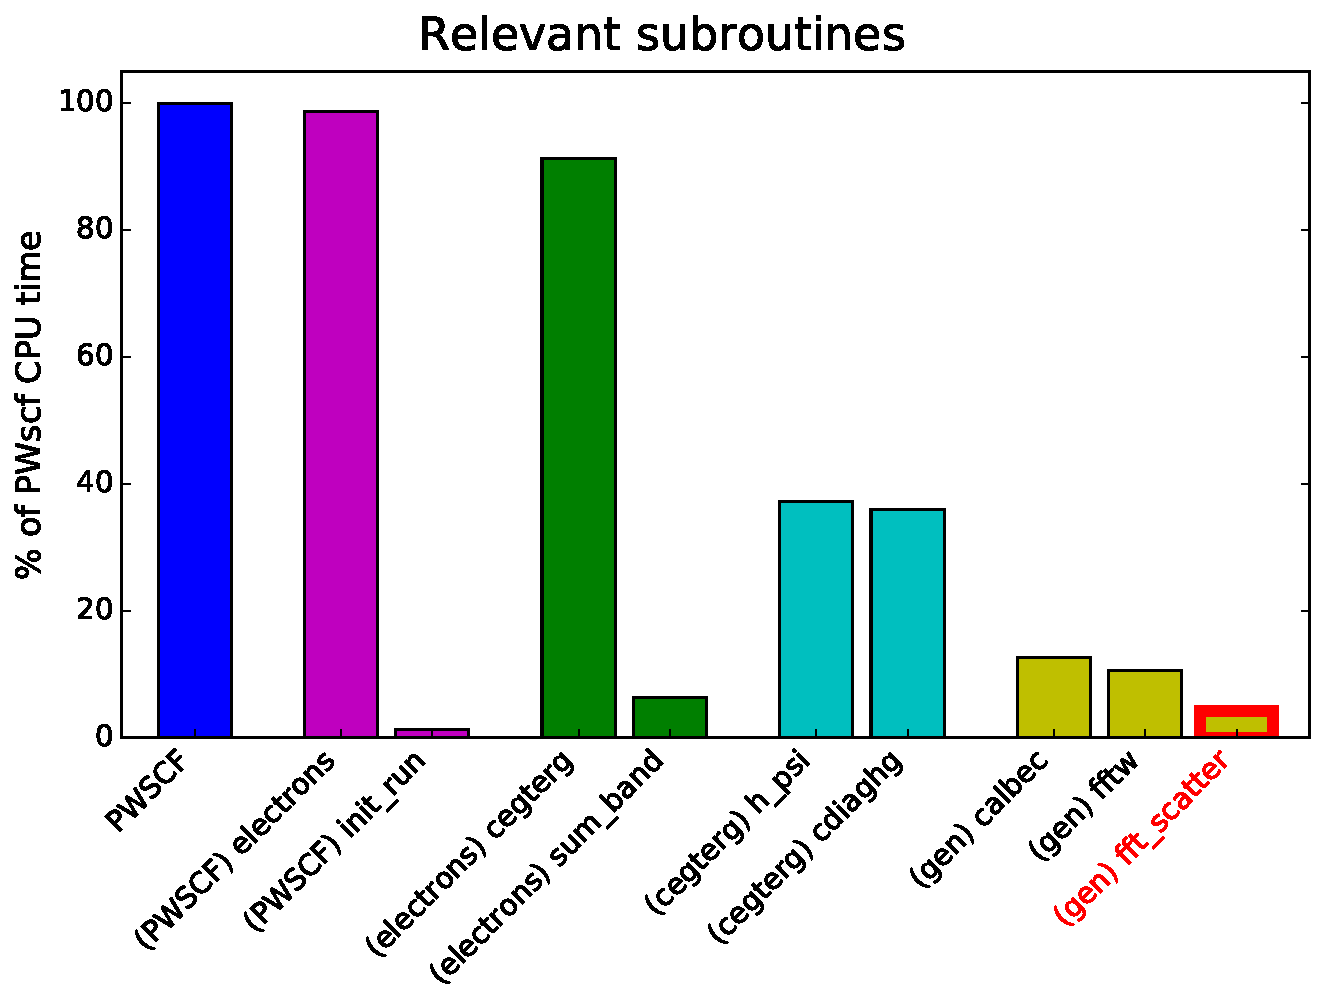
\includegraphics[height=0.5\textheight, width=1\textwidth]{beam_relevant_subroutines_fft_scatter.pdf}	
				}
				\end{center}    	
    	\end{columns}

    \end{minipage}
}

\end{frame}


% ********** slide 6 *****************}

\begin{frame}{Architetture computazionali}

\vspace{-1cm}

\begin{columns}
	\column{0.5\textwidth}
	\begin{block}{CINECA Galileo cluster}
		\begin{itemize}
			\item Architettura multicomputer
			\item Ogni nodo indipendente
			\item 16 core per nodo divisi su due socket
			\item Interconnect Infiniband
		\end{itemize}
	\end{block}

	\column{0.5\textwidth}
			\begin{center}
				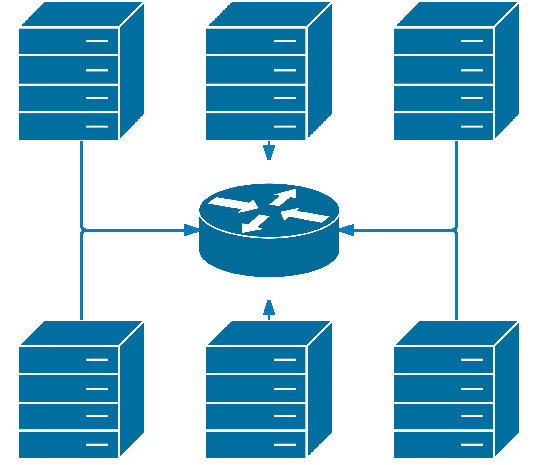
\includegraphics[height=0.4\textheight]{beam_galileo_schema.pdf}
			\end{center}
\end{columns}

\begin{columns}
	\column{0.5\textwidth}
	\begin{block}{Sgi Altix UV2000 CC-NUMA}
		\begin{itemize}
			\item Architettura multiprocessore
			\item Unica macchina a memoria condivisa
			\item 8 core per nodo NUMA
			\item 64 core totali
		\end{itemize}
	\end{block}
	
	\column{0.5\textwidth}
	\begin{center}
			\begin{center}
				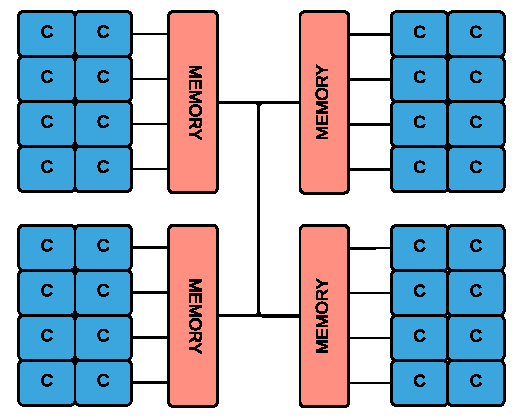
\includegraphics[height=0.4\textheight]{beam_numa_schema.pdf}
			\end{center}
	\end{center}
	
\end{columns}

\end{frame}


% ********** slide 9 *****************}

\section{Risultati}
\subsection{Risultati}

\begin{frame}{Risultati}
\begin{columns}
	\visible<1->{
	\column{0.5\textwidth}
		\begin{block}{Indipendenti dall'architettura}
			\begin{itemize}
				\item Su singolo nodo
				%\item Bassa parallelizzazione
				\item Basso numero di core
				\item No interconnect
			\end{itemize}
		\end{block}
	}
	\visible<1->{
	\column{0.5\textwidth}
		\begin{block}{Dipendenti dall'architettura}
			\begin{itemize}
				\item Nodi multipli
				\item Alta parallelizzazione
				%\item Alto numero di core
				\item Interconnect o memoria condivisa
			\end{itemize}
		\end{block}
	}
\end{columns}
\begin{center}
	\visible<2->{
	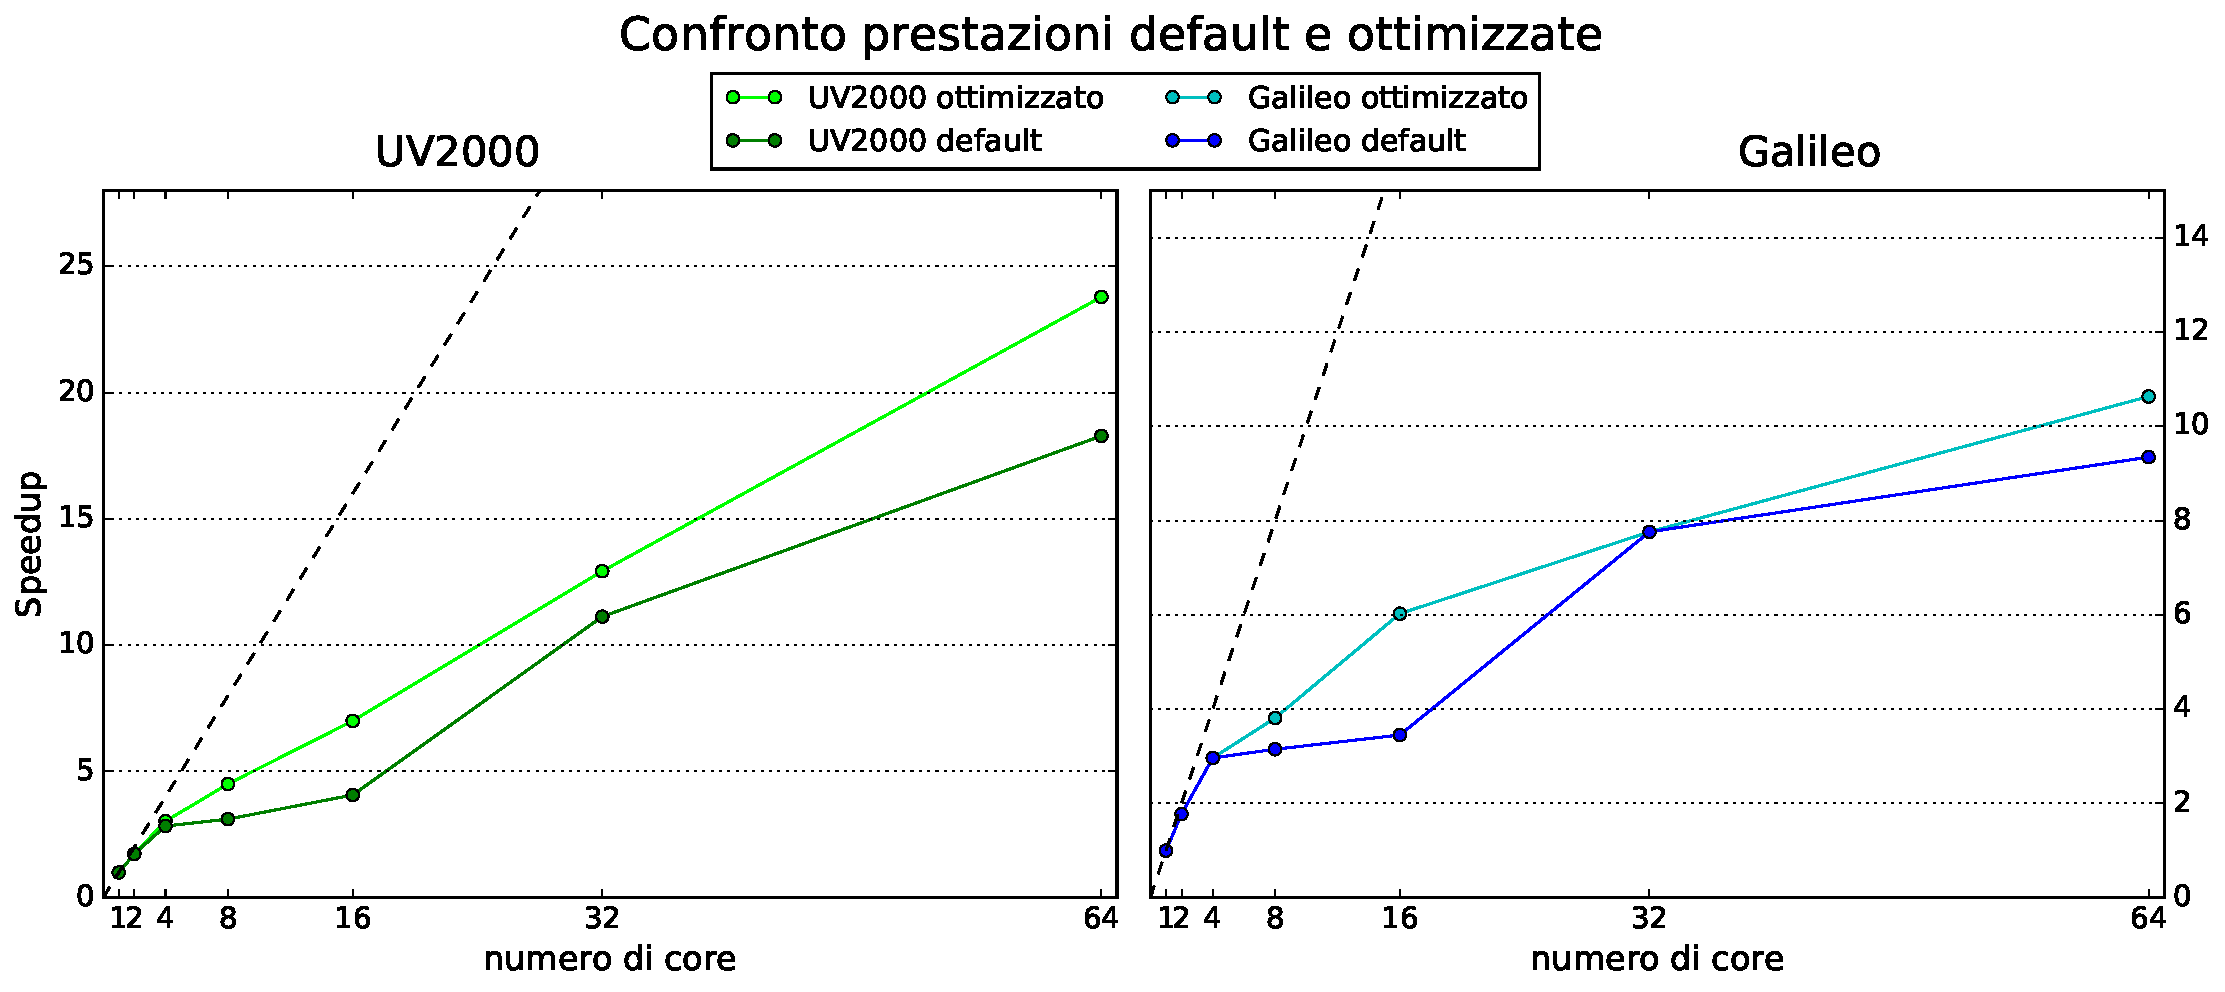
\includegraphics[height=0.6\textheight]{beam_results_arch_comparison.pdf}	
	}
\end{center}
\end{frame}



% ********** slide 10 *****************}

\begin{frame}{Indipendenti dall'architettura}

\begin{columns}[c]

\column{0.5\textwidth}
\parbox[c]{0.5\linewidth}
{
\begin{center}
	\only<1>{
	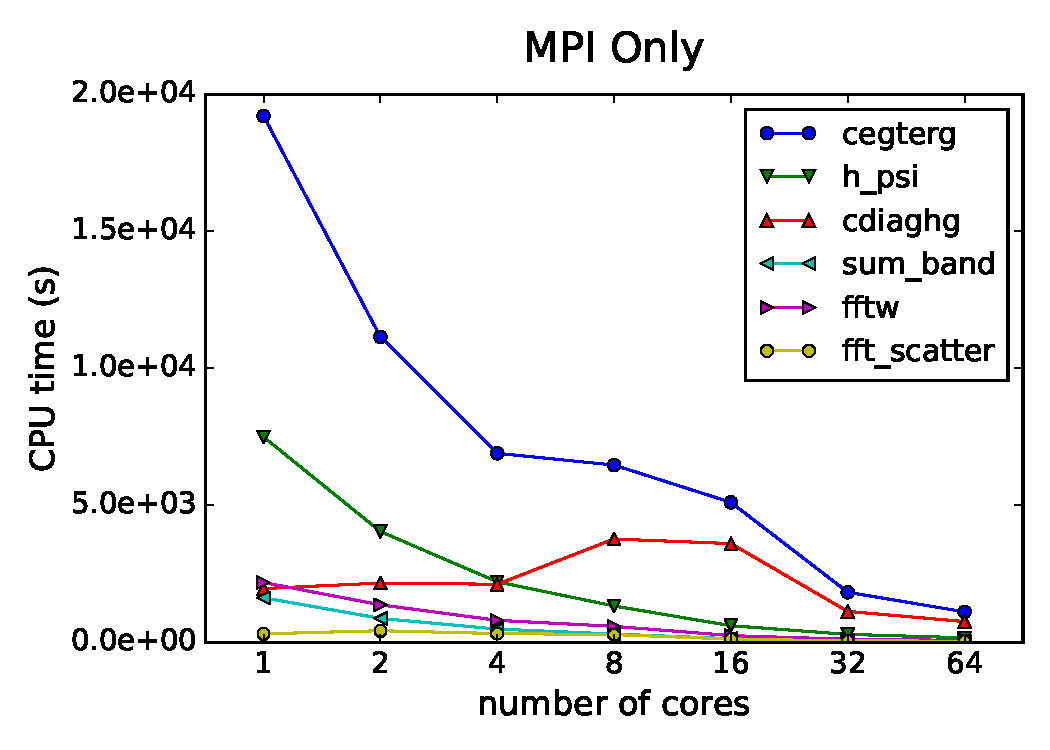
\includegraphics[width=1\textwidth, height=0.5 \textheight]{beam_threads_MPIonly.pdf}	
	}
	\only<2,3>{
	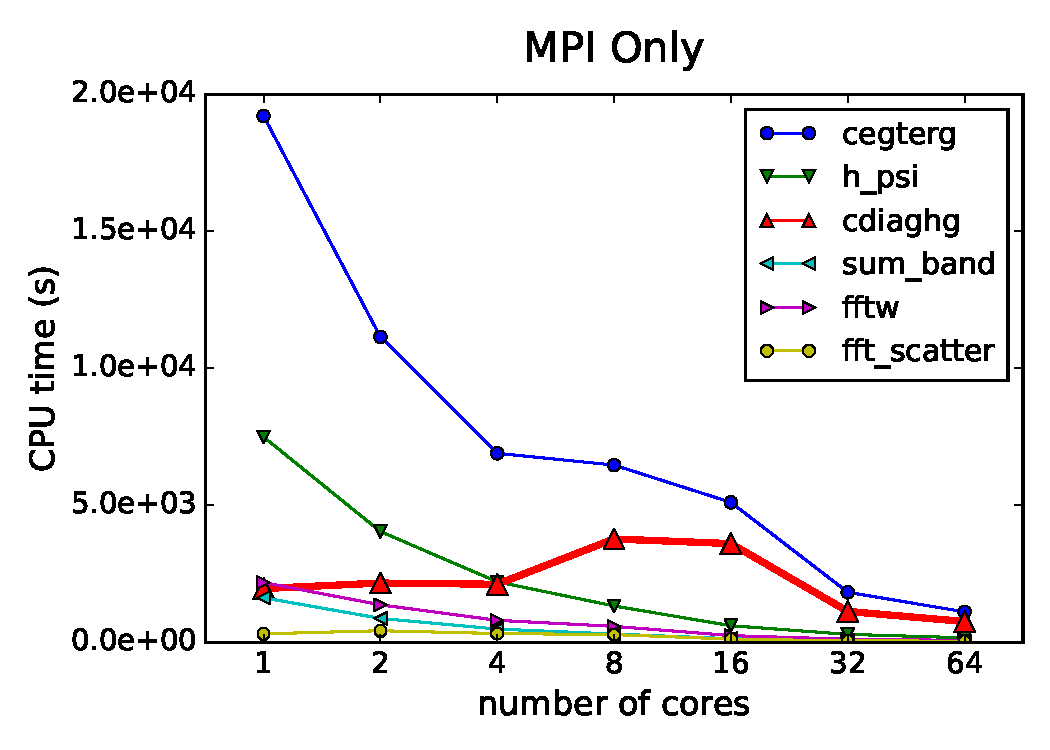
\includegraphics[width=1\textwidth, height=0.5 \textheight]{beam_threads_MPIonly_cdiaghg.pdf}	
	}
	%\only<3>{
	%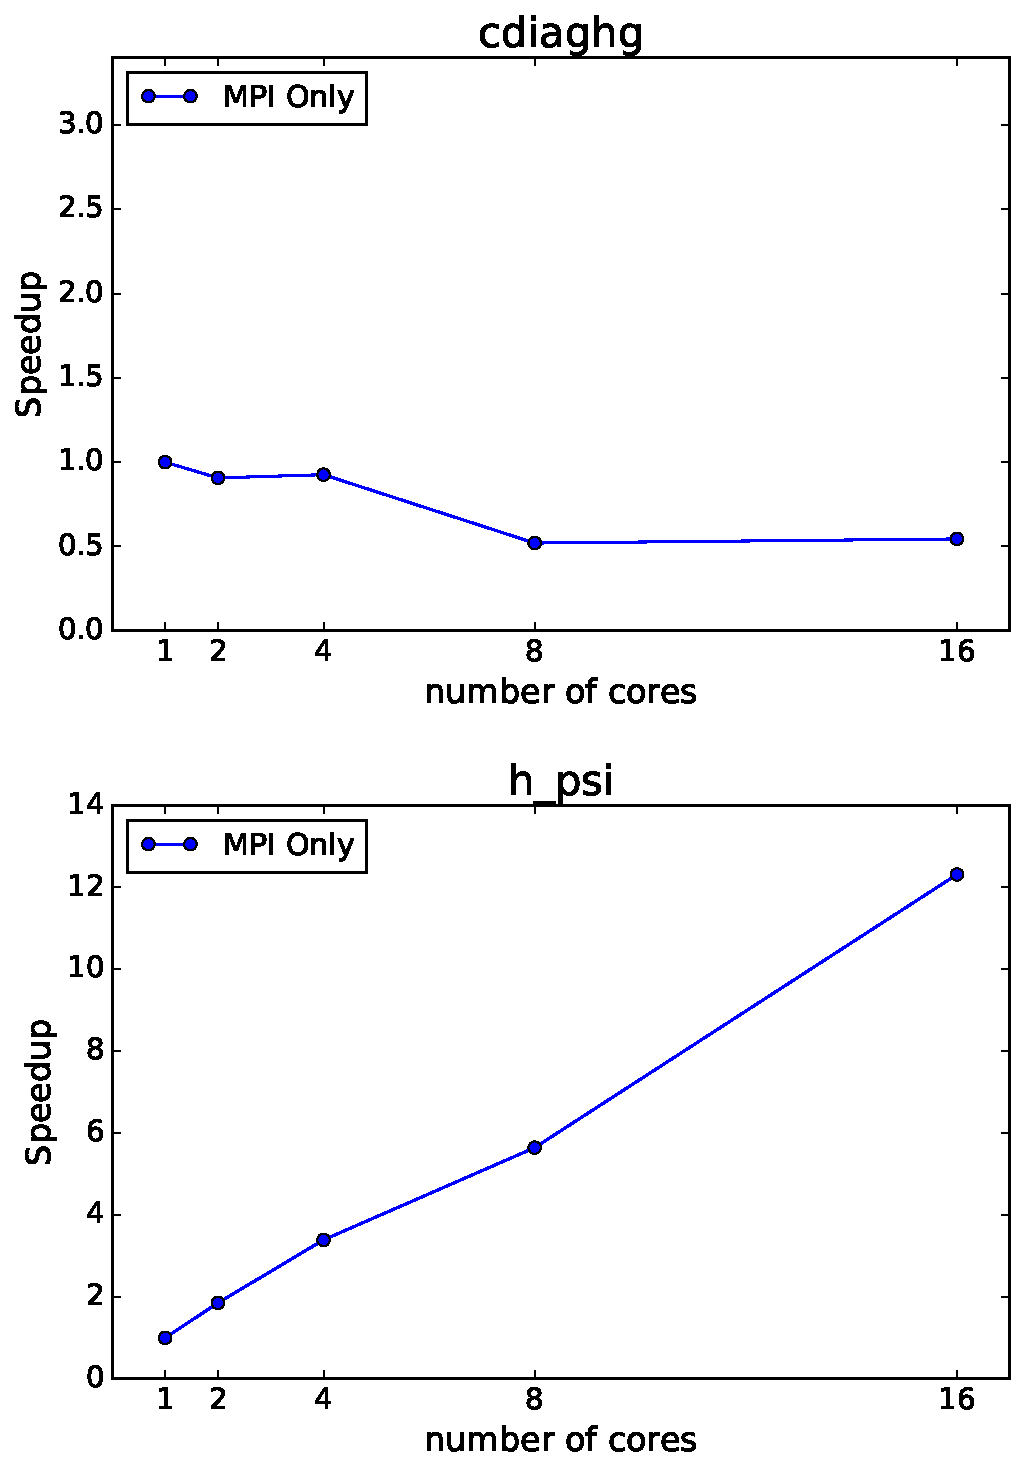
\includegraphics[width=0.9\textwidth, height=0.85 \textheight]{beam_threads_subroutines_MPI.pdf}	
	%}
	\only<4->{
	\vspace{-1cm}
	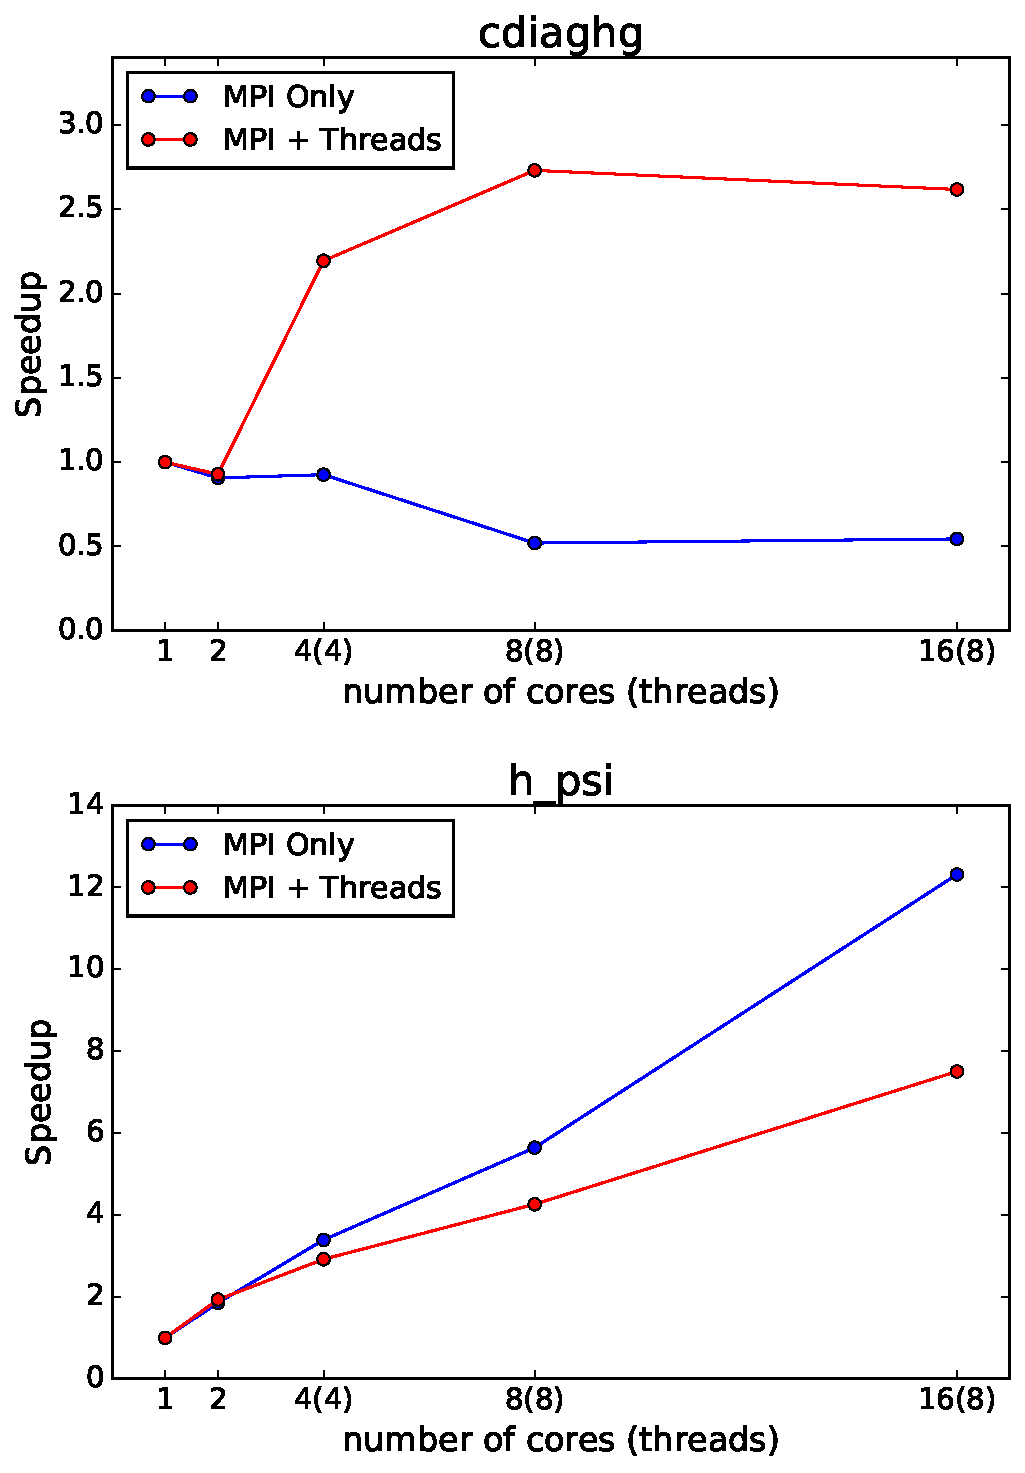
\includegraphics[width=0.9\textwidth, height=0.85 \textheight]{beam_threads_subroutines_MPI_threads.pdf}	
	}
\end{center}
}

\column{0.5\textwidth}
\begin{center}
\begin{overlayarea}{\linewidth}{\textheight}


	\begin{block}{Comportamento}
		\begin{itemize}
			\item<1-> MPI: parallelizzazione multiprocesso a memoria distribuita
			\item<2-> Diagonalizzazione ScaLapack poco performante
			\item<3-> Alternativa: uso MKL Threads
			\item<4-> Valutazione Hamiltoniana rallenta ma diagonalizzazione \`e pi\`u efficiente
			\item<5-> Risultato?
		\end{itemize}
	\end{block}

\end{overlayarea}
\end{center}

\end{columns}


\end{frame}


% ********** slide 11 *****************}
\begin{frame}{Indipendenti dall'Architettura}
	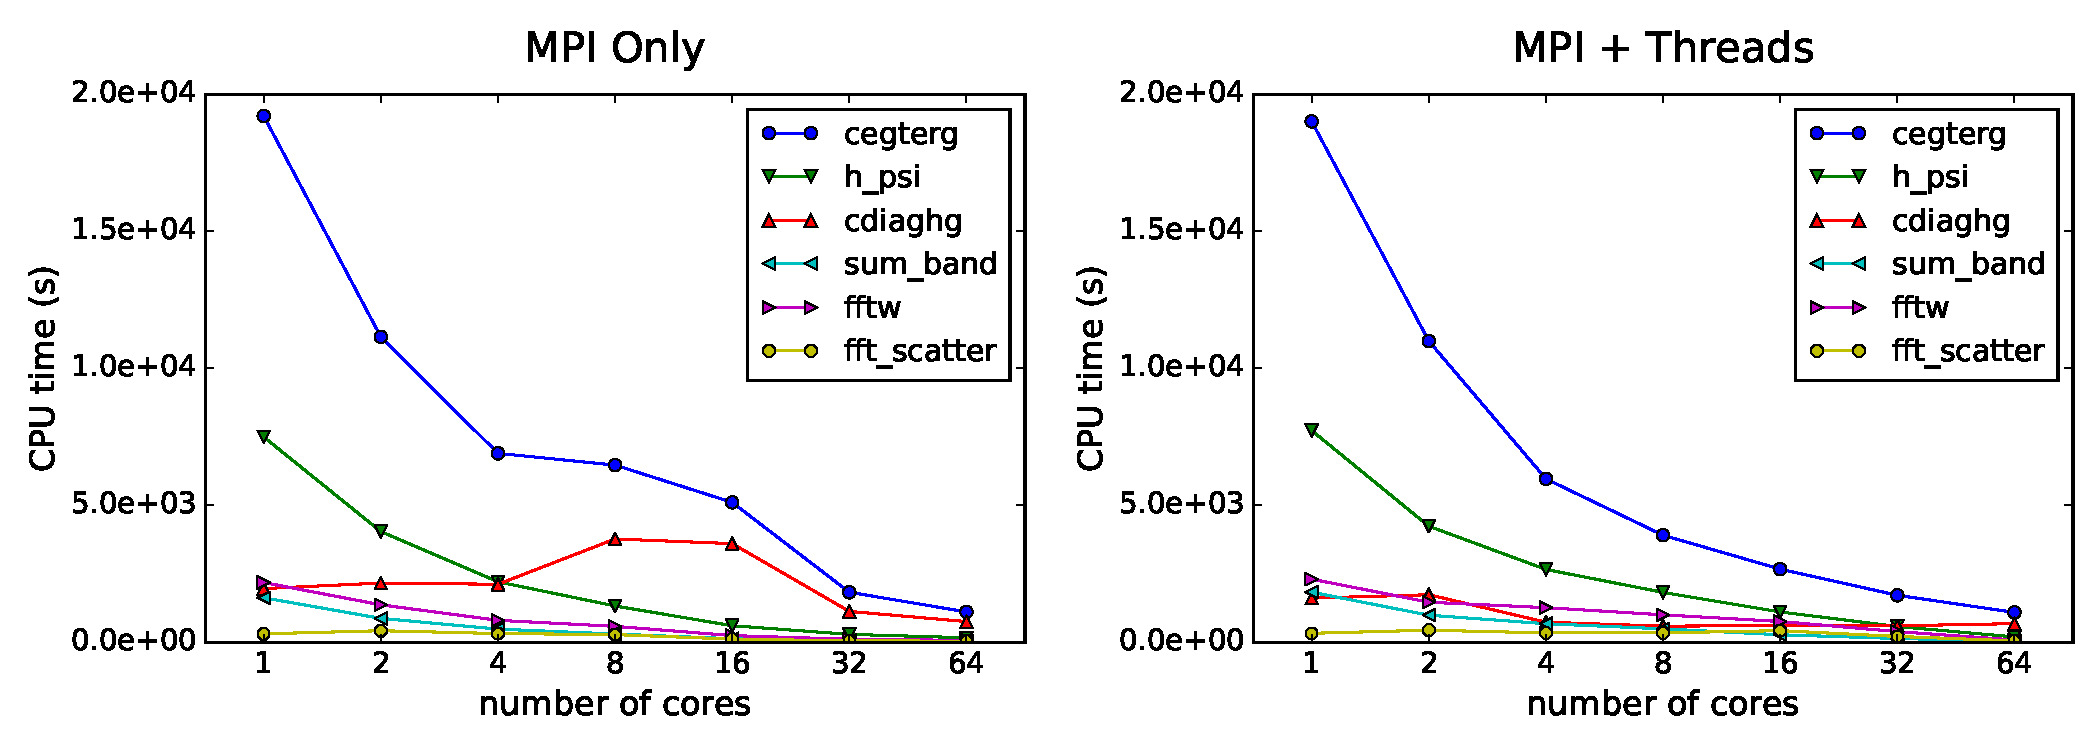
\includegraphics[width=1\textwidth]{threads_comparison.pdf}	
\end{frame}



% ********** slide 12 *****************}
\begin{frame}{Dipendenti dall'architettura}
\begin{columns}
	\column{0.5\textwidth}
			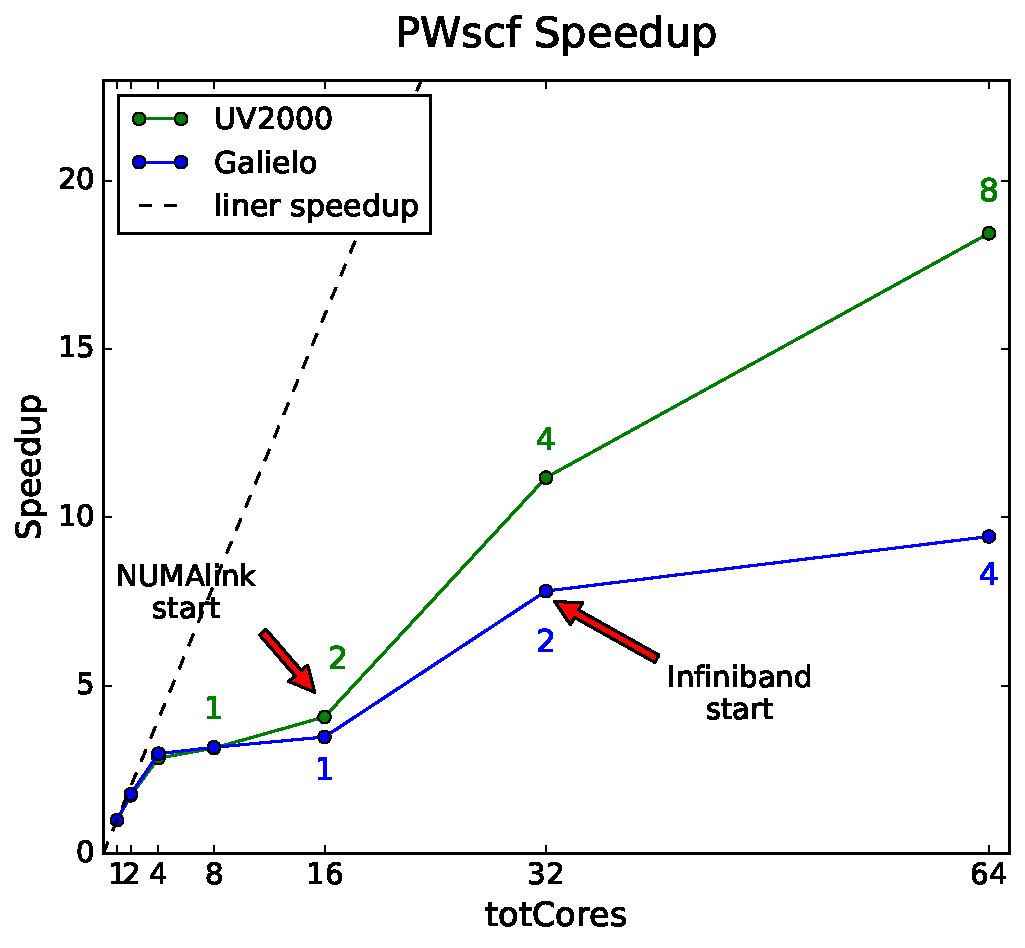
\includegraphics[width=1\textwidth]{beam_arch_global.pdf}			
	\column{0.5\textwidth}
		\begin{block}{Confronto Architetture}
			\begin{itemize}
				\item UV2000 miglior speedup
				\item Differenza cresce all'aumentare dei nodi
				\item Comunicazione	
			\end{itemize}
		\end{block}
\end{columns}
\end{frame}



% ********** slide 14 *****************}
\begin{frame}{Dipendenti dall'architettura}
\begin{columns}
	\column{0.6\textwidth}
		\begin{center}			
			\vspace{-1cm}
			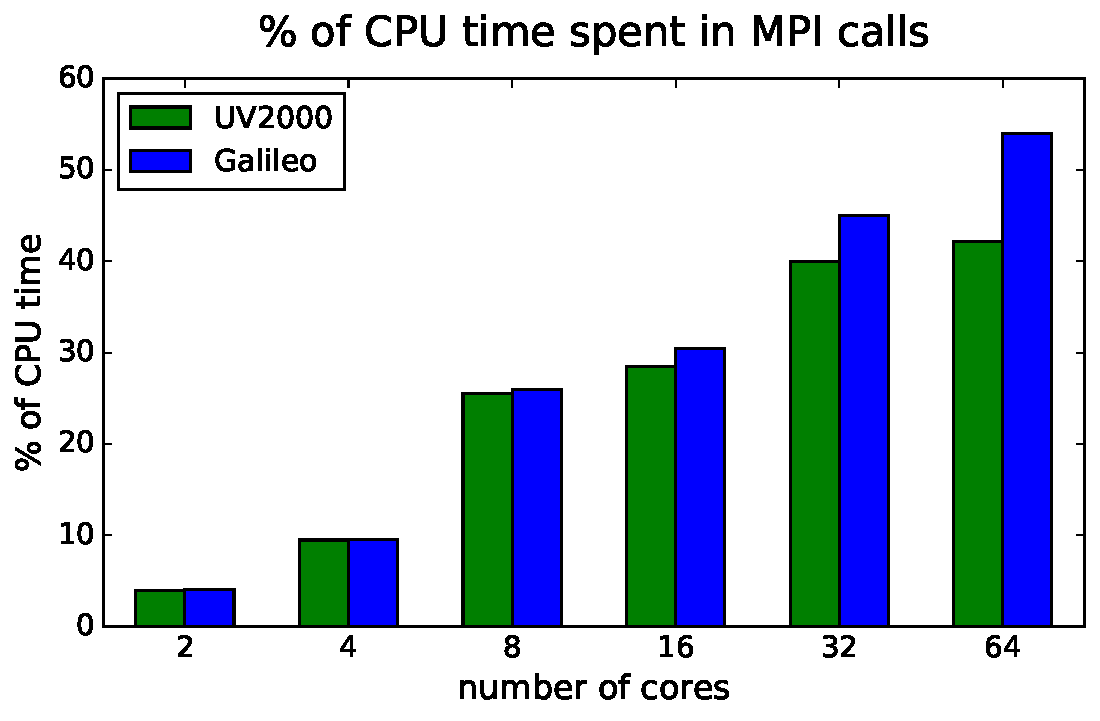
\includegraphics[width=1\textwidth]{arch_mpi_perc.pdf}			
		\end{center}
	\column{0.4\textwidth}
		\begin{overlayarea}{\linewidth}{\textheight}
		\begin{block}{Comunicazione}
			\begin{itemize}
				\item<1-> Ruolo comunicazione cresce sensibilmente
				\item<2-> Oltre il singolo nodo UV2000 \`e pi\`u efficiente.
				\item<3-> Indicativo ma non giustifica la differenza in prestazioni.\\Comunicazione ScaLAPACK non \`e profilata!
			\end{itemize}		
		\end{block}

		\end{overlayarea}
\end{columns}

\end{frame}

% ********** slide 15 *****************}
\begin{frame}{Dipendenti dall'architettura}

	\begin{center}
		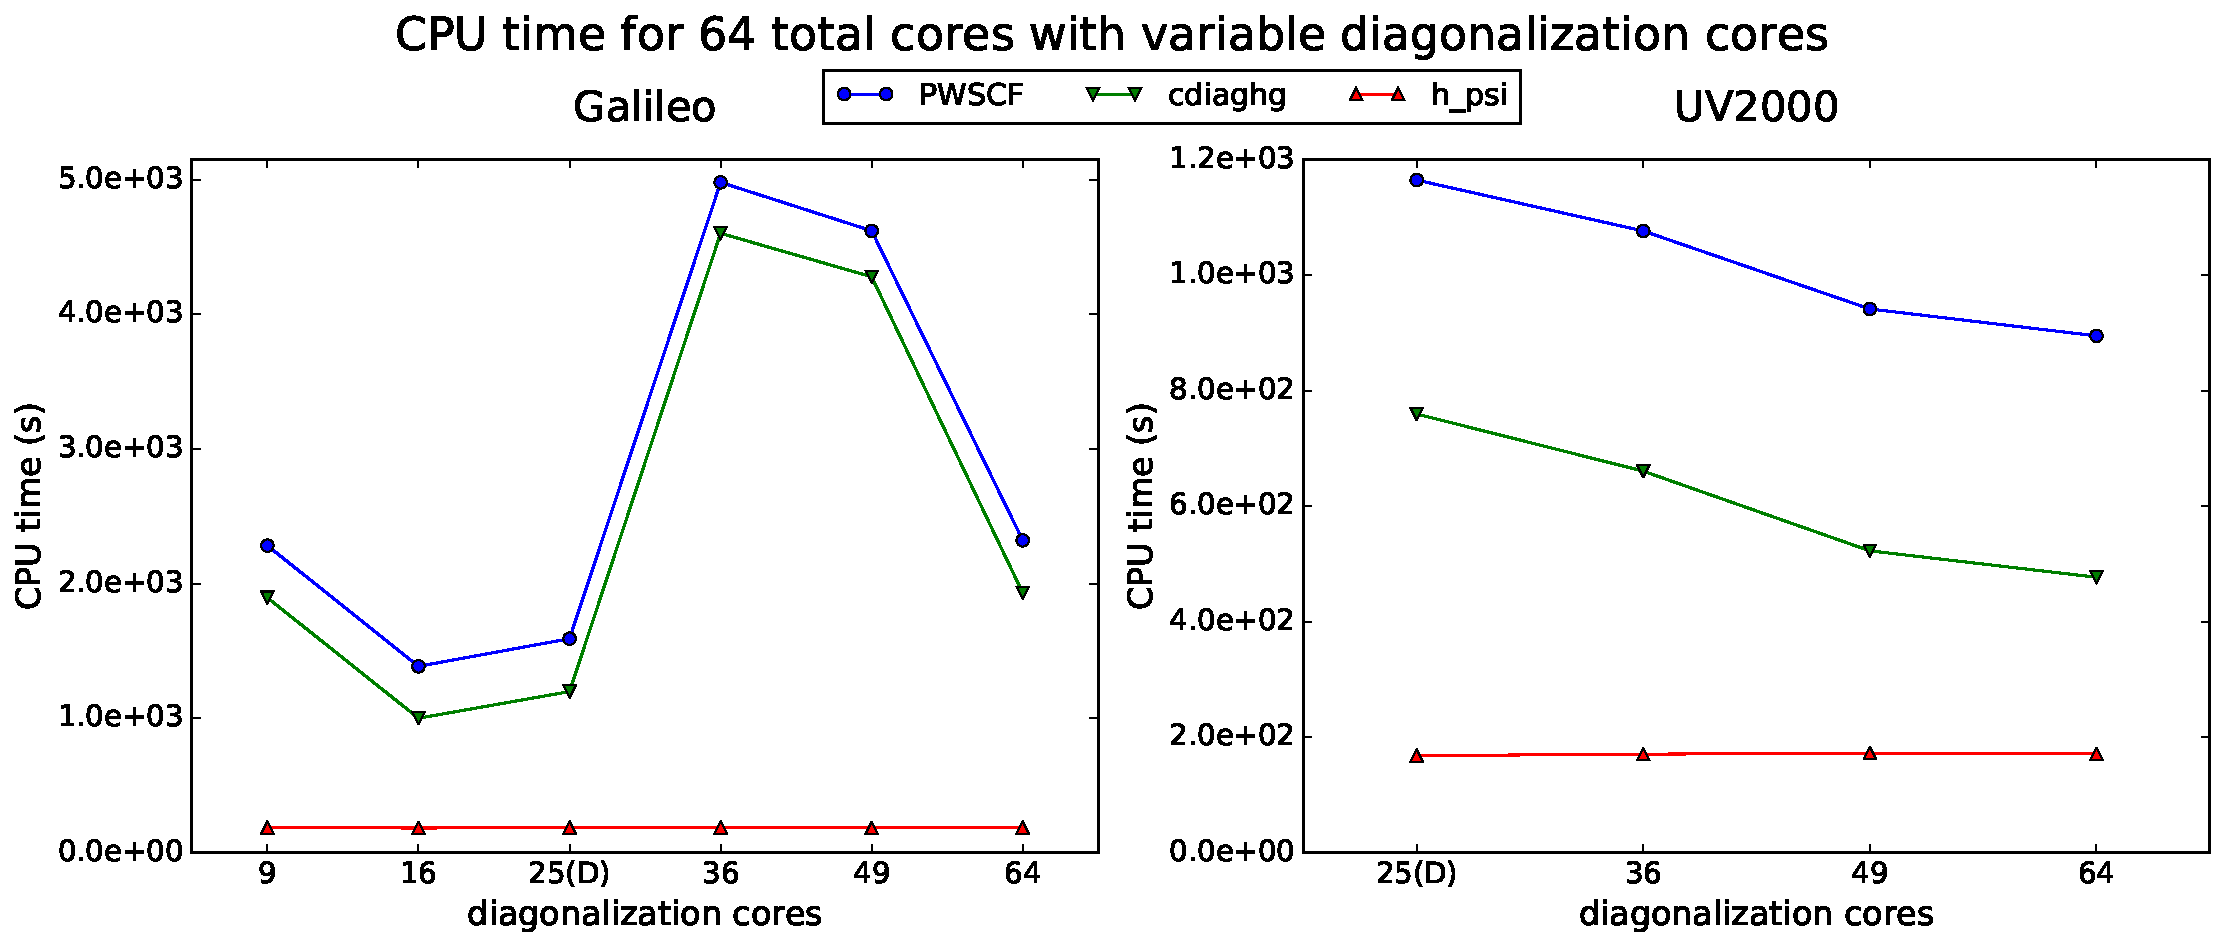
\includegraphics[width=0.95\textwidth]{beam_ndiag_64.pdf}			
	\end{center}

	\begin{overlayarea}{\linewidth}{\textheight}
	\vspace{-0.6cm}
	\begin{columns}
	\hspace{0.1\textwidth}
		\column{0.45\textwidth}
		\visible<1->
		{
		\begin{center}
			\begin{block}{Galileo}
				\begin{itemize}
				\item migliori prestazioni diminuendo i core
				\item miglior risultato con tutti i processi su singolo nodo
				\end{itemize}							
			\end{block}			
		\end{center}
		}
		
		\column{0.45\textwidth}
		\visible<2->
		{
		\begin{center}
			\begin{block}{UV2000}
			\begin{itemize}
				\item migliori prestazioni aumentando i core
				\item miglior risultato occupando tutti i processori
				\item sconsigliato in letteratura
				\end{itemize}	
			\end{block}		
		\end{center}
		}
	\end{columns}
	\end{overlayarea}


\end{frame}


% ********** slide 16 *****************}
\begin{frame}{Dipendenti dall'architettura}
\vspace{-0.5cm}

	\begin{columns}
	\column{0.33\textwidth}
	\begin{center}	
		50 Atomi\\
		\CO \\
		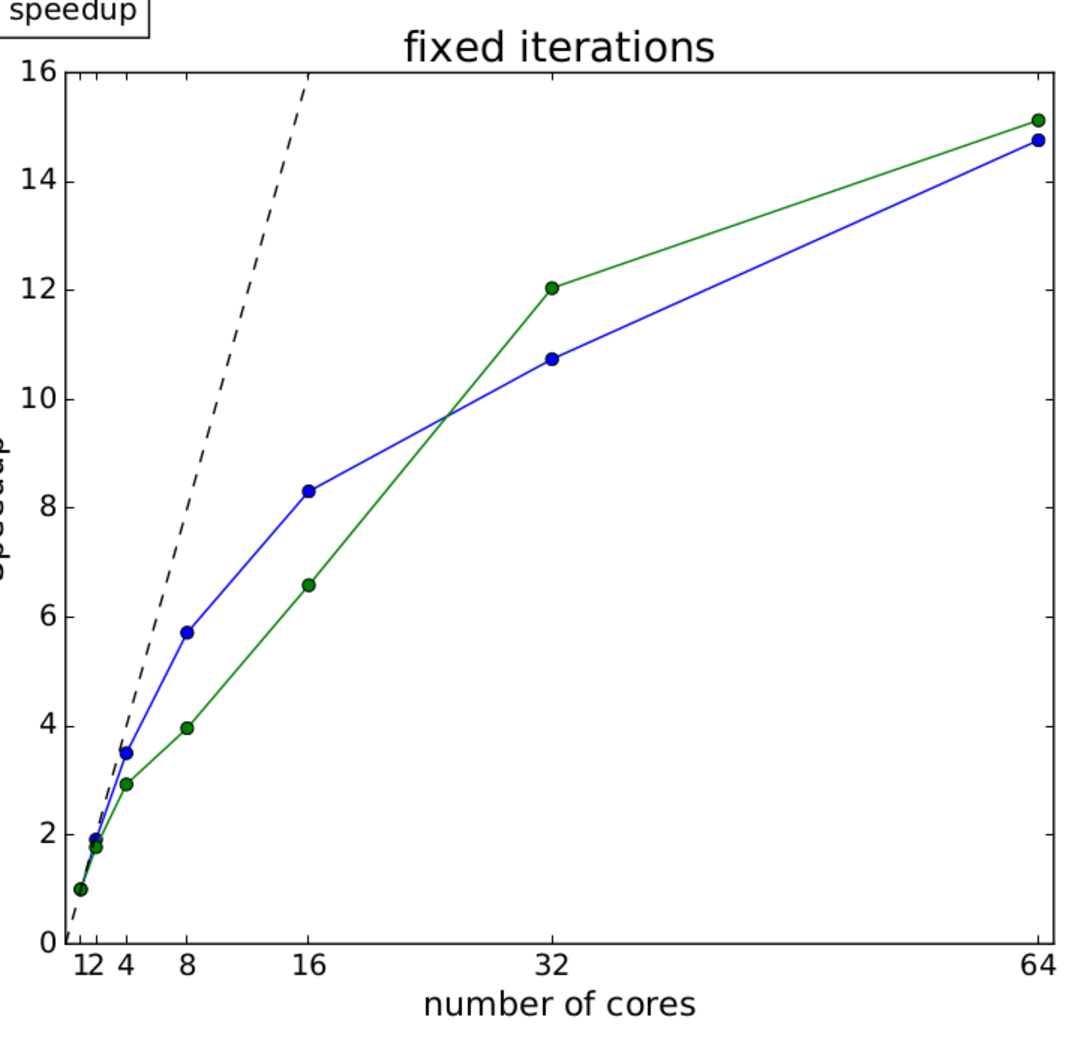
\includegraphics[width=0.95\textwidth]{beam_concl_co3.pdf}	\\		
		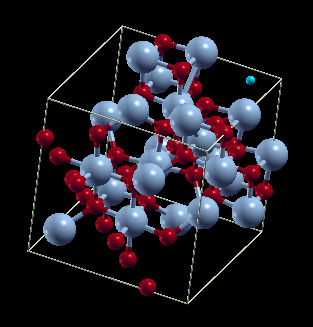
\includegraphics[height=3cm]{beam_co3.png}
	\end{center}

	
	\column{0.33\textwidth}
	\begin{center}	
		100-150 Atomi\\
		Au Surf 112 - TiO\textsubscript{2}\\
		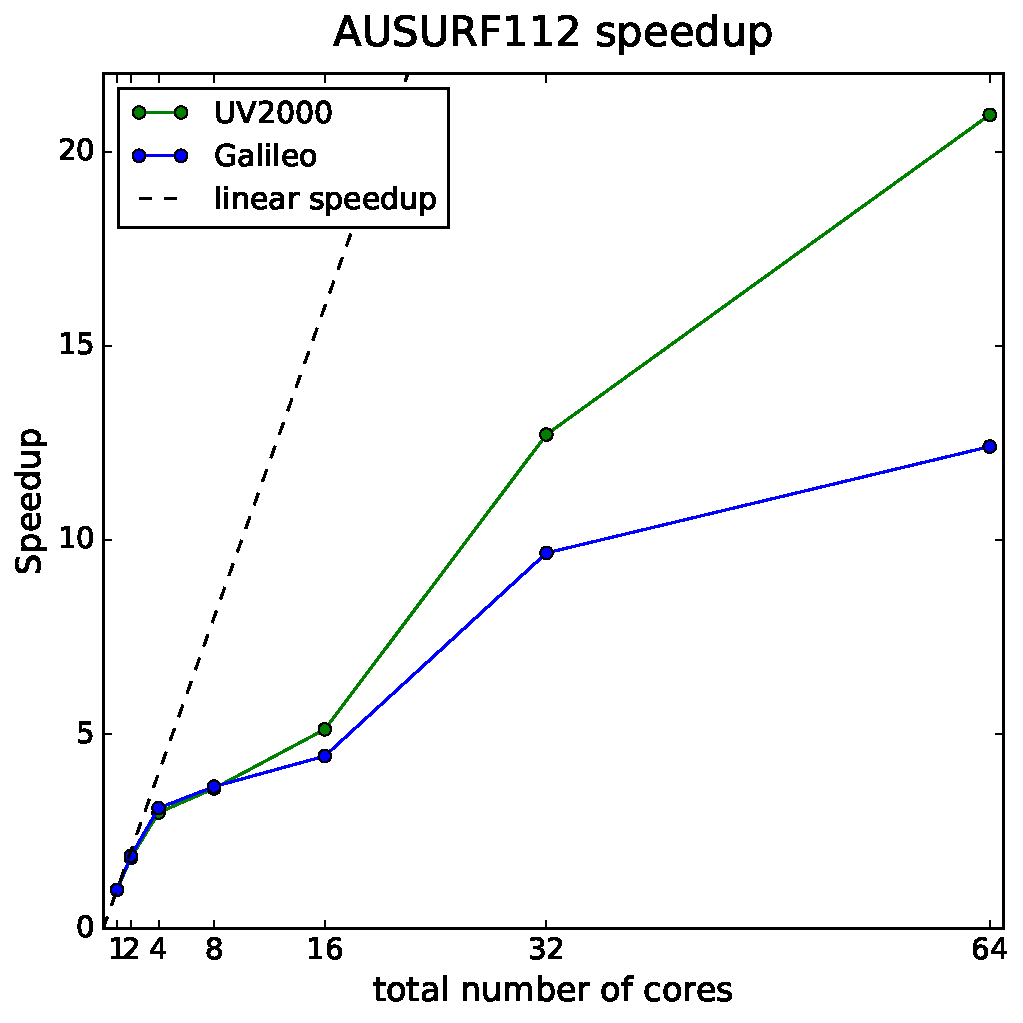
\includegraphics[width=0.95\textwidth]{concl_ausurf.pdf}\\		
		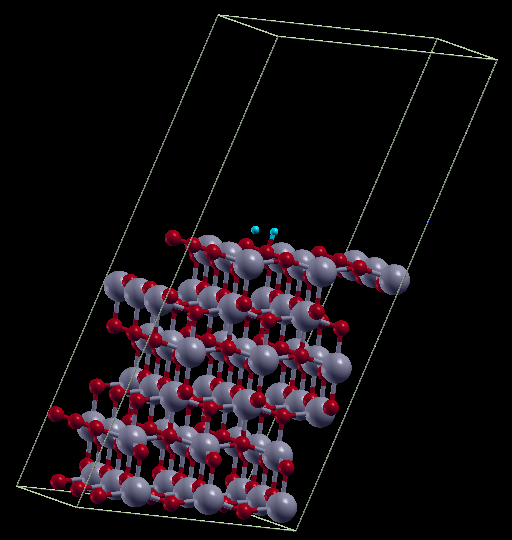
\includegraphics[height=3cm]{titania_crystal.png}
	\end{center}	
			
	\column{0.33\textwidth}

	\begin{center}	
		250-300 Atomi\\
		Cristallo Organico\\
		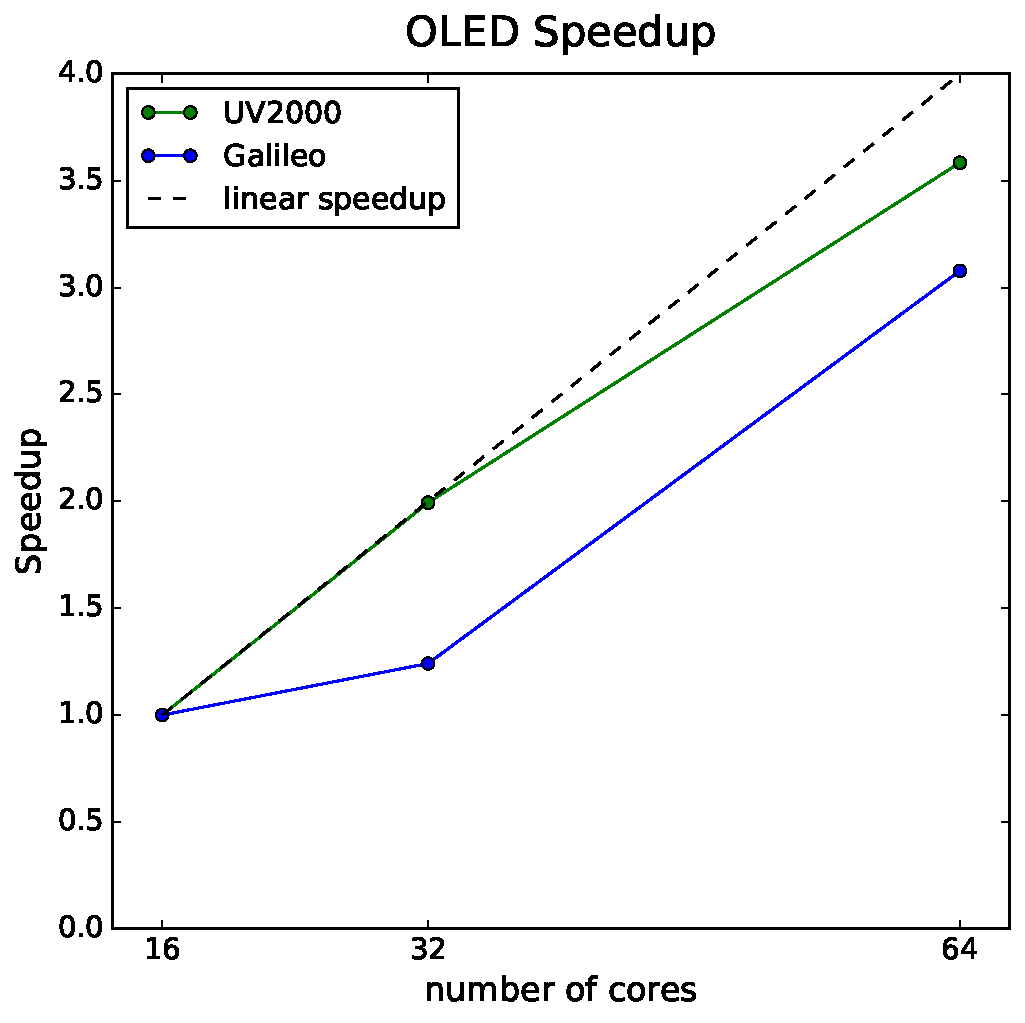
\includegraphics[width=0.95\textwidth]{concl_oled.pdf}	\\	
		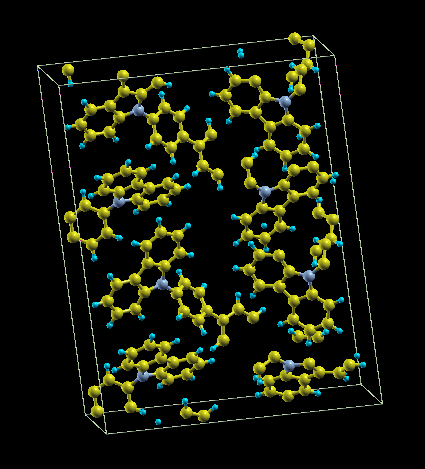
\includegraphics[height=3cm]{beam_cbp.png}
	\end{center}		
	
	\end{columns}
	

\end{frame}





% ********** Conclusioni *****************}

\section{Conclusioni}
\subsection{Conclusioni}

\begin{frame}{Conclusioni}
\vspace{-0.07\textheight}
\begin{center}
	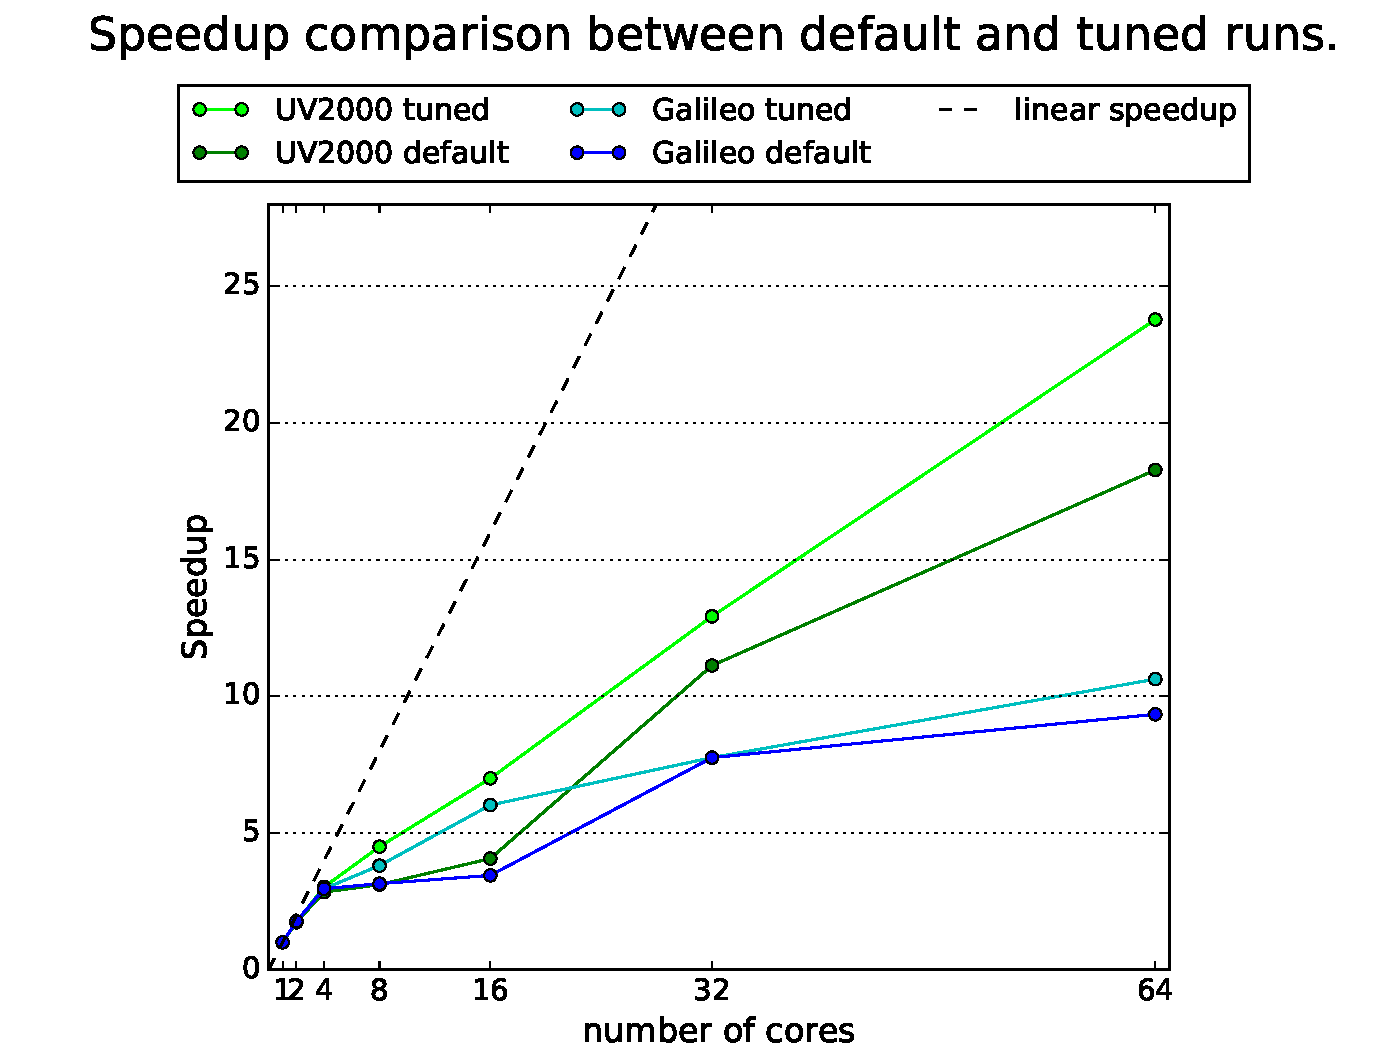
\includegraphics[height=0.6\textheight]{beam_last_slide.pdf}	
\end{center}


\pause
Abbiamo trovato strategie di ottimizzazione adatte a vari scenari:

\begin{itemize}

	\item L'utilizzo dei thread \`e interessante in scenari HTC e in casi di sovraccarico risorse condivise.
	\pause
	\item L'architettura a memoria condivisa \`e chiaramente pi\`u performante su sistemi medio-grandi in ambito altamente parallelizzato.
	\pause
	\item Il peso della diagonalizzazione (trascurato in letteratura) \`e importante e le strategie per ottimizzarla variano a seconda dell'architettura computazione.
\end{itemize}
\end{frame}



\begin{frame}{Sviluppi futuri}
	\begin{itemize}
		\item Studio comportamento su nuove architetture Knight Landing (Intel MIC), CINECA Marconi.
		\item Miglior stima dei processori per diagonalizzazione.
		\item Algoritmi di moltiplicazione matrici alternativi (SUMMA).
		\item Aumento di risorse computazionali.
		\item Combinazione NUMA + GPU.
		\item Analisi predittiva per miglior ottimizzazione.
	\end{itemize}
	\vspace{1cm}
	\begin{columns}
		\column{0.15\textwidth} 
		\begin{center}
			
\includegraphics[width=1.2\textwidth]{beam_qe_logo.jpg}
		\end{center}
		\column{0.15\textwidth} 
		\begin{center}
			
\includegraphics[width=0.8\textwidth]{beam_e4_logo.png}
		\end{center}
		\column{0.15\textwidth} 
		\begin{center}
			
\includegraphics[width=0.8\textwidth]{beam_eap_logo.jpg}
		\end{center}
		\column{0.15\textwidth} 
		\begin{center}
			
\includegraphics[width=\textwidth]{beam_istm_logo.png}
		\end{center}
		\column{0.15\textwidth} 
		\begin{center}
			
\includegraphics[width=\textwidth]{beam_cnr_logo.png}
		\end{center}
		\column{0.15\textwidth} 
		\begin{center}
			
\includegraphics[width=\textwidth]{beam_lcm_logo.png}
		\end{center}											
	\end{columns}
\end{frame}

\appendix	
\begin{frame}

\end{frame}


% ********** Backup *****************}

\begin{frame}{Scaling Funzioni} %ex slide 13
\begin{columns}
	\column{0.66\textwidth}
		\begin{center}			
			\vspace{-1cm}
			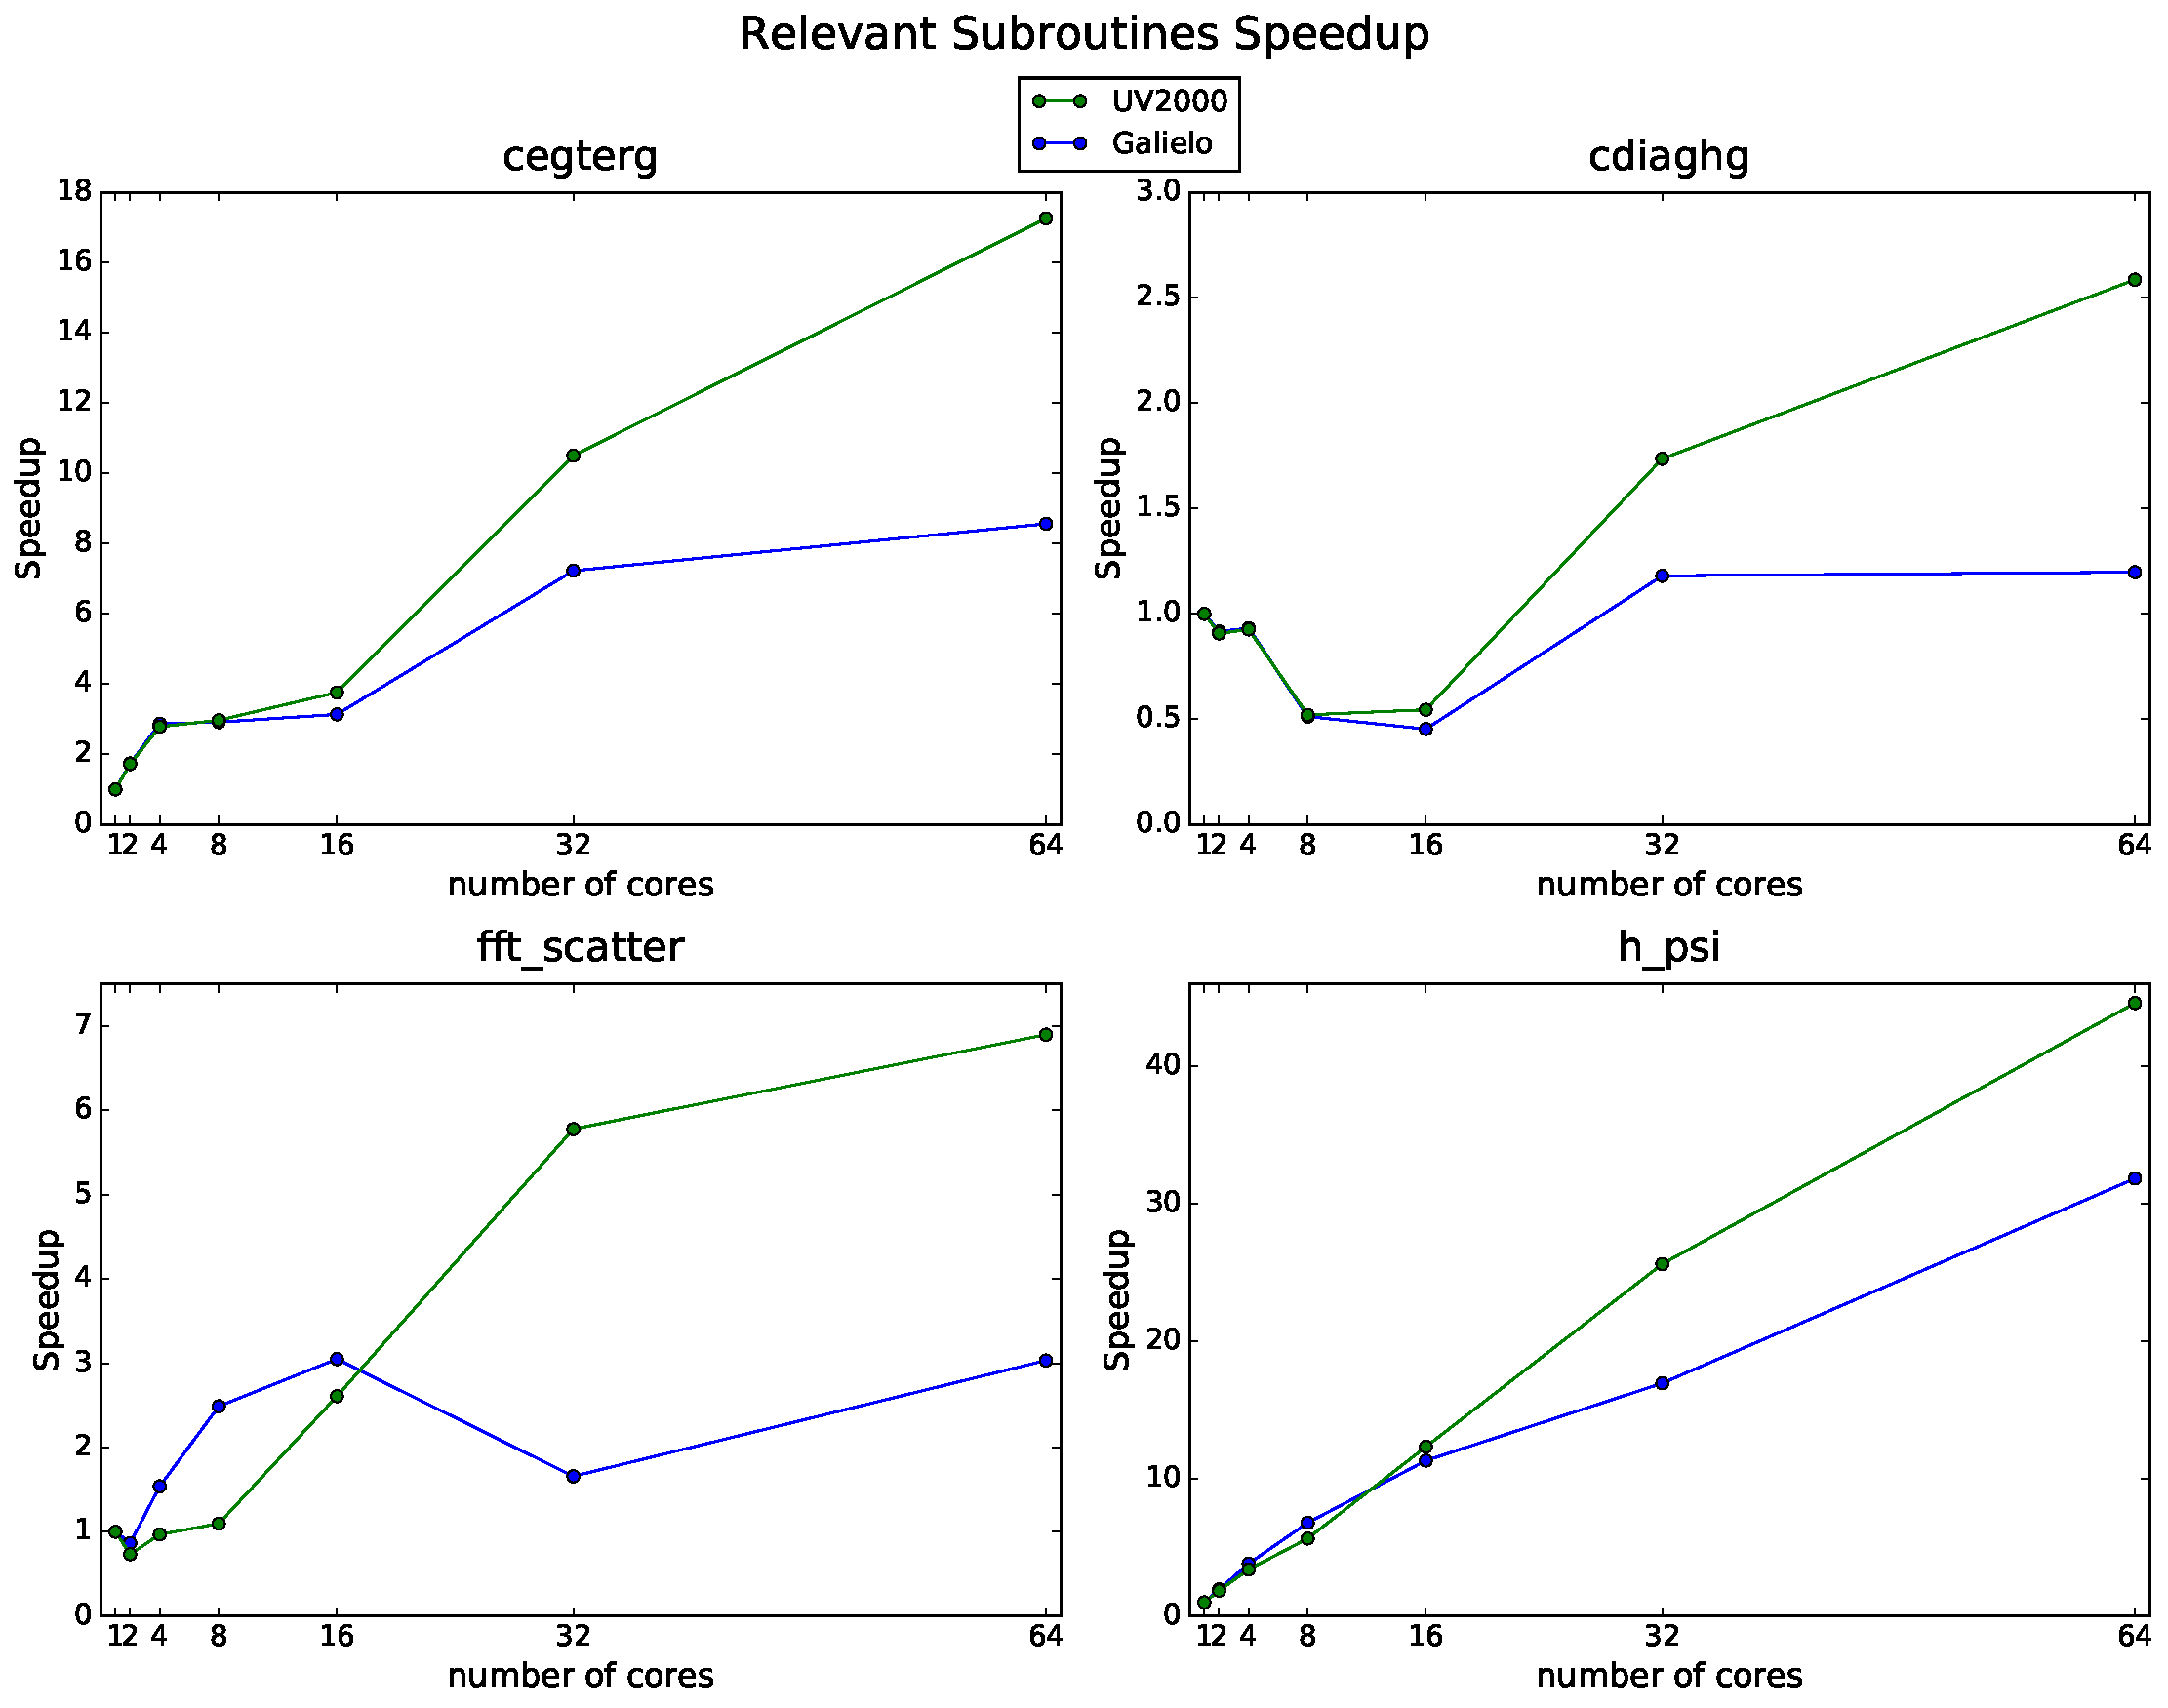
\includegraphics[width=1.1\textwidth]{beam_arch_subroutines.pdf}			
		\end{center}
	\column{0.33\textwidth}
		\begin{overlayarea}{\linewidth}{\textheight}
		\begin{block}{Funzioni}
			\begin{itemize}
				\item Equazioni di Kohn-Sham
				\item Diagonalizzazione Hamiltoniana
				\item Valutazione Hamiltoniana
				\item Distribuzione griglia
				\item Comunicazione?
			\end{itemize}		
		\end{block}

		\end{overlayarea}
\end{columns}

\end{frame}


\begin{frame}{Azzeramento}
\begin{itemize}
	\item allocazione totale risorse
	\item riduzione massima I/O su disco
	\item process pinning (NUMA)
	\item uso di migliori librerie
\end{itemize}
\begin{center}
	\includegraphics[height=0.5\textheight]{cpuwalltime.pdf}	
\end{center}
\end{frame}


\begin{frame}{DFT1}
	\begin{align}
		E[\dens] = T[\dens] + V_{ee}[\dens] + \int \dens v_{ion}(\erre) \dd{\erre} \\
			\mu_{HK} = v(\erre) + \frac{\var{E_{HK}[\dens]}}{\var{\dens}}
	\end{align}
	\begin{align}
&\hat{H}_{ref} = \sum_{i} \hat{h}_i^{KS} ;
&\hat{h}_i^{KS} = - \frac{\nabla^{2}_{i}}{2} + v(\erre)_{ref} .
\end{align}

\begin{align}
		E[\dens] &= 	T_{ref}[\dens] + J[\dens] + \int \dens v_{ion}(\erre) \dd{\erre}\\
			 &+ \lbrace
			 	T[\dens] + V_{ee}[\dens] - 
			 	\left( 
			 		T_{ref}[\dens] + J[\dens] 
			 	\right)
			 \rbrace
\end{align}
	
\begin{align}
	&\mu_{KS} = \frac{\var{T_{ref}[\dens]}}{\var{\dens}}  + v_{eff}(\erre); &v_{eff}(\erre) = v_{ion}(\erre) + v_{h}(\erre) + v_{xc}(\erre)
\end{align}
\begin{equation}
 \lbrace  - \frac{1}{2} \nabla^2+ v_{eff}(\erre) \rbrace 	\psi_{j}^{KS}(\erre) = \varepsilon_{j}^{KS} 	\psi_{j}^{KS}(\erre)
\end{equation}
\end{frame}

\begin{frame}{DFT2}
\begin{equation}
	v_{eff} = v_{ion} + v_{h} + v_{xc},
\end{equation}
\begin{equation}
	\tilde{v}_{ion}(\mf{G}) = \sum_{\mf{G}} f_{ps}^{sp}(G) e^{i \mf{G} \cdot \mf{R}_{\alpha}},
\end{equation}
\begin{equation}
	\tilde{v}_{h}(\mf{G}) = \frac{\tilde{\rho}(\mf{G})}{G^2 \varepsilon_{0}},
\end{equation}
\begin{equation}
	v_{xc}(\erre) =	\frac{\var{E_{xc}[\dens]}}{\var{\dens}}
\end{equation}
\begin{equation}
	v_{eff}(\erre) = IFFT\{\tilde{v}(\mf{G})\}(\erre) + IFFT\{\tilde{v}_{h}(\mf{G})\}(\erre) + v_{xc}(\erre).
\end{equation}
\\
\begin{equation}
	E[\dens] = \sum_{j}\varepsilon^{KS}_{j} - E_{h}[\dens] - \int \dens v(\erre) \dd{\erre}+ E_{xc}[\dens].
\end{equation}
\begin{equation}\label{eq:HartreeEnergy}
E_{h}[\dens] = \frac{1}{2} \iint \frac{\rho(\mathbf{r_{1}}) \rho(\mathbf{r_{2}}) }{r_{12}} \dd{\mathbf{r_1}} \dd{\mathbf{r_2}} = J[\dens]
\end{equation}


\end{frame}



\begin{frame}{Criterio di convergenza}
\begin{equation}
	\Delta\dens = \densin - \densout.
\end{equation}
QE considers the terms in $E[\dens + \Delta\dens] - E[\dens ]$ quadratical in $\Delta\dens$ 
\begin{align}
	\Delta E &= E[\dens + \Delta\dens] - E[\dens ] \\
	&\simeq \frac{e^2}{2} \iint \frac{\Delta\rho(\erre) \Delta\rho(\erre')}{\mid \erre - \erre' \mid} \dd{\erre} \dd{\erre'}\\
	 &= \int \Delta\dens \Delta v_{h}(\erre') \dd{\erre},
\end{align}

\end{frame}


\begin{frame}{\texttt{h\_psi} e FFT}
\begin{align*}
	IFFT[f(\GI)] &= \sum_{j}^{N_x} \sum_{k}^{N_y} \sum_{l}^{N_z} f^{\GI}_{jkl}
		exp \left[i \frac{2\pi}{N_x}ju \right] 
		exp \left[i \frac{2\pi}{N_y}kv \right] 
		exp \left[i \frac{2\pi}{N_x}lw \right] \\
		[u,v,w] &= \mf{q} \\
		[j,k,l] &= \mf{b}_i.
\end{align*}
	\begin{center}
		\includegraphics[width=0.6\textwidth]{h_psi.pdf}
	\end{center}
\end{frame}



\begin{frame}{Complessita Numerica}

\begin{table}[h]
\centering


\begin{tabular}{llll}
\textbf{Routine}            & \textbf{Description} & \textbf{Calls} & \textbf{Complexity} \\
\hline
\hline
\\[0pt]
\texttt{init\_run} &  \begin{tabular}[c]{@{}l@{}} first approximation of\\ $\dens$, $\{u_{kj}\}$ and $v_{eff}$. \end{tabular} & 1 per PWscf run &  \begin{tabular}[c]{@{}l@{}} $v_{eff} : \bigO(N log (N) )$ \\ Diag $: \bigO(N_{b}^3)$ \end{tabular} \\[20pt]
\texttt{c\_bands}  & Diagonalization of $\mf{H}^{KS}$ & 1 per SCF step & $\bigO(N_{b}^3)$           
\\[20pt]
\texttt{h\_psi}    & Compute $\mf{H}^{KS} \ket{u_{kj}}$  & $N_{b}$ per Davidson step     & $\bigO(N log (N))$            
\\[20pt]

\texttt{sum\_bads} & \begin{tabular}[c]{@{}l@{}} Calculate $\densout$,$\varepsilon_{j}$\\ and occupations \end{tabular} & 1 per SCF step      &  $\bigO(N log (N))$  
\\[20pt]
\hline         

\end{tabular}
\caption{Summary of the most important routines in \QE}
\label{tab:coreRoutines}
\end{table}
\end{frame}

\begin{frame}

\begin{table}[]
\centering
\begin{tabular}{lc}
\hline
\multicolumn{1}{|l|}{\textbf{Size}} & \multicolumn{1}{l|}{\textbf{Description}}                                                                                                                        \\ \hline
\multicolumn{1}{|l|}{$N_{R}$}       & \multicolumn{1}{l|}{Number of $\mf{R}$ points in the real grid}                                                                                                  \\ \hline
\multicolumn{1}{|l|}{$N_{G}$}       & \multicolumn{1}{l|}{Number of $\GI$ points in the reciprocal grid}                                                                                               \\ \hline
\multicolumn{1}{|l|}{$N_{G}^{PW}$}  & \multicolumn{1}{l|}{\begin{tabular}[c]{@{}l@{}}Number of $\GI$ points in the reciprocal grid associated to \\ plane waves below the cutoff energy\end{tabular}} \\ \hline

                                    & \multicolumn{1}{l}{}                                                                                                                                             \\ \cline{2-2} 
\multicolumn{1}{l|}{}               & \multicolumn{1}{c|}{\textbf{Relationships}}                                                                                                                      \\ \cline{2-2} 
\multicolumn{1}{l|}{}               & \multicolumn{1}{c|}{$N_{R} = N_{G} = N = N_x N_y N_z$}                                                                                                                         \\ \cline{2-2} 
\multicolumn{1}{l|}{}               & \multicolumn{1}{c|}{$N_{G}^{PW} < N$}                                                                                                                       \\ \cline{2-2} 
\multicolumn{1}{l|}{}               & \multicolumn{1}{c|}{\textbf{Estimate for a 100 atom system}}                                                                                                                       \\ \cline{2-2} 
\multicolumn{1}{l|}{}               & \multicolumn{1}{c|}{ $N_{b} \simeq \frac{1}{2} N_{e^{-}} \simeq 10^3~;~ N_{G}^{PW} \simeq 10^{6} ~;~ N \simeq 10^7 $}                                                                                                                       \\ \cline{2-2} 
                                    &                                                                                                                                                                  \\ \cline{2-2} 
\multicolumn{1}{l|}{}               & \multicolumn{1}{c|}{\textbf{Computational cost of every Fast Fourier Transform}}                                                                                           \\ \cline{2-2} 
\multicolumn{1}{l|}{}               & \multicolumn{1}{c|}{$\mathcal{O}(N log (N))$}                                                                                                                    \\ \cline{2-2} 
\end{tabular}
\caption{Summary of typical dimensions between direct and reciprocal grid}
\label{tab:FFTSummary}
\end{table}

\end{frame}

\begin{frame}{Comparazione con HF}

\begin{table}[h]
\centering
\begin{tabular}{l|l|ll|l|}
\cline{2-2} \cline{5-5}
                                    & \textbf{DFT-PW}        &                       &                    & \textbf{HF-Gaussian} \\ \cline{1-2} \cline{4-5} 
\multicolumn{1}{|l|}{\textbf{FFT}}  & $\bigO(N_{b}N ln(N) )$ & \multicolumn{1}{l|}{} & $\mf{H}_{ij}$ & $\bigO(N_{gauss}^4)$ \\ \cline{1-2} \cline{4-5} 
\multicolumn{1}{|l|}{\textbf{DIAG}} & $\bigO(N_{b}^3)$       & \multicolumn{1}{l|}{} & \textbf{DIAG}      & $\bigO(N_{b}^3)$     \\ \cline{1-2} \cline{4-5} 
\end{tabular}
\caption{Comparison of computational complexity between DFT method using plane waves and HF method using Gaussian orbitals. $\mf{H}_{ij}$ stands for the evaluation of the Hamiltonian(mainly the Fock operator), \textbf{DIAG} is the cost of the diagonalization, $N_b$ is the number of bands, $N_{gauss}$ is the number of Gaussian orbitals in the basis set.}
\label{tab:HF-DFTComp}
\end{table}
\end{frame}


\begin{frame}{Iterazioni Variabili}
	\begin{center}
		\includegraphics[width=0.9\textwidth]{concl_final_comparison.pdf}
	\end{center}
\end{frame}

\begin{frame}
	\begin{center}
		\includegraphics[width=\textwidth]{threads_overall.pdf}
	\end{center}
\end{frame}

\begin{frame}{Dinamica SCF}
	\begin{center}
		\includegraphics[width=0.9\textwidth]{iterstats.pdf}
	\end{center}
	
	
\begin{table}[hhh!]
\begin{center}
\begin{tabular}{r|cccc}
\toprule
cores &        mean iteration time(s) &         st-dev(s) &   relative error(\%) &   number of iterations \\
\midrule
1  &  676 &  201 &  29 &  43 \\
2  &  363 &  118 &  32 &  42 \\
4  &  207 &   68 &  33 &  70 \\
8  &  204 &  102 &  50 &  86 \\
16 &  154 &  109 &  71 &  55 \\
32 &   80 &   44 &  55 &  36 \\
64 &   58 &   35 &  60 &  50 \\
\bottomrule
\end{tabular}
\end{center}
\caption{Iterations statistics for self consistent calculation on variable number of cores.}
\label{tab:iterations}
\end{table}

\end{frame}





\end{document}
